\documentclass[11pt]{amsart}
\pdfoutput=1
\usepackage[letterpaper,margin=1in]{geometry}
\usepackage[dvipsnames]{xcolor}
\usepackage{amssymb,mathrsfs,mathtools,esint,graphicx,nicefrac}
\newcommand{\nf}{\nicefrac}
\usepackage[square]{natbib}
\AddToHook{env/thebibliography/begin}{\interlinepenalty=10000}
\usepackage[citecolor=PineGreen,colorlinks=true,linkcolor=RoyalBlue,urlcolor=BrickRed,pdfstartview=FitV]{hyperref}
\newtheorem{proposition}{Proposition}[section]
\newtheorem{theorem}[proposition]{Theorem}
\newtheorem{lemma}[proposition]{Lemma}
\newtheorem{corollary}[proposition]{Corollary}
\newtheorem{conjecture}[proposition]{Conjecture}
\theoremstyle{definition}
\newtheorem{assumption}[proposition]{Assumption}
\theoremstyle{remark}
\newtheorem{remark}[proposition]{Remark}
\numberwithin{equation}{section}
\newcommand{\E}{\mathbb E}
\newcommand{\Q}{\mathbb Q}
\newcommand{\R}{\mathbb R}
\newcommand{\N}{\mathbb N}
\newcommand{\Zd}{\mathbb Z^d}
\renewcommand{\a}{\mathbf a}
\renewcommand{\b}{\mathbf b}
\newcommand{\ahom}{\overline{\mathbf a}}
\newcommand{\Div}{\operatorname{Div}}
\newcommand{\cA}{\mathcal A}
\renewcommand{\epsilon}{\varepsilon}
\title[Quantitative Einstein relation]{Quantitative Einstein relation for reversible diffusions in a random environment}
\hypersetup{pdftitle={Quantitative Einstein relation for reversible diffusions in a random environment},pdfauthor={Ahmed Bou-Rabee and Ruizhe Xu}}
\author{Ahmed Bou-Rabee}
\address{Department of Mathematics, University of Pennsylvania, Philadelphia, PA 19104}
\email{ahmedb@sas.upenn.edu}
\author{Ruizhe Xu}
\address{School of Mathematical Sciences, Zhejiang University, Hangzhou, China}
\email{ruizhexu.math@gmail.com}
\begin{document}
\begin{abstract}
A reversible diffusion in a random environment, pushed by a small constant force, moves with an asymptotic velocity. The Einstein relation states that, as the force tends to zero, the ratio of this velocity to the force magnitude converges to the diffusivity matrix of the unforced diffusion, evaluated in the force direction. Gantert, Mathieu and Piatnitski (2012) proved this relation. We prove the sharp rate of convergence. If the coefficient field is uniformly elliptic, the potential is bounded, and both are Lipschitz, jointly stationary and have a finite range of dependence, then in every dimension $d\geq2$ the difference is at most a constant times the force magnitude. We construct examples attaining this order. The proof uses quantitative homogenization on the length scale of the inverse force.
\end{abstract}
\maketitle

\section{Introduction}\label{sec.intro}

A particle diffusing in a disordered medium, subjected to a small constant force, eventually drifts at an asymptotic velocity. To leading order, this velocity is a linear function of the force; the proportionality matrix is called the \textbf{mobility}. The \textbf{Einstein relation} predicts that the mobility equals the diffusivity matrix of the unforced particle. The relation admits several mathematical formulations, depending on the order in which the small-force and long-time limits are taken (see Section~\ref{ss.background}). We work with the formulation of \citet*{Einstein2012gantert} for reversible diffusions in a random environment: the velocity is first defined at a fixed force, and its ratio to the force magnitude is then compared, as the force tends to zero, with the diffusivity matrix evaluated in the force direction. We prove that, in every dimension $d\geq2$, the difference between the two is at most a constant times the force magnitude (Theorem~\ref{t.main}). This rate is optimal: for each $d\geq2$, there are environments in which the difference is of exactly this order (Proposition~\ref{sharp.example}).

\begin{figure}[ht]
\centering
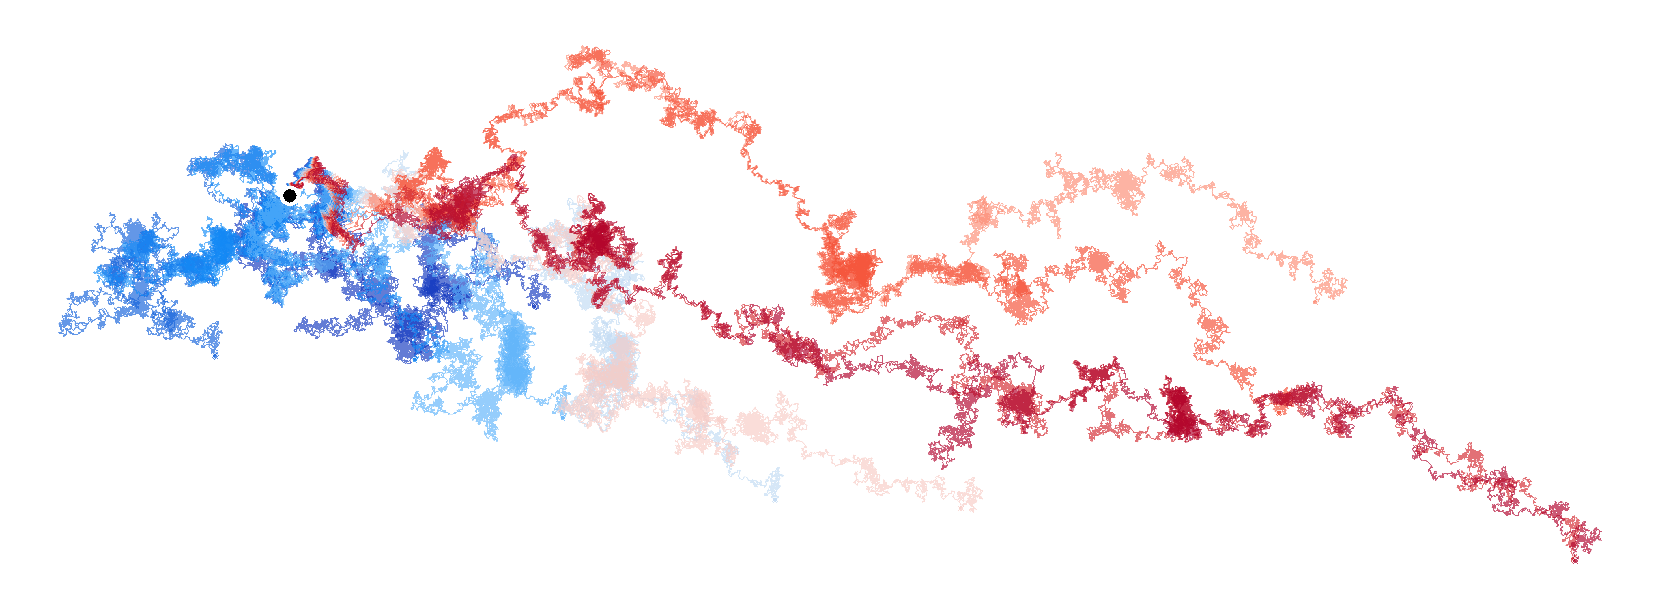
\includegraphics[width=\textwidth]{einstein_paths.pdf}
\caption{Sample paths of Brownian motions with drift~$\lambda e_1$, started from a common origin (black dot), with $\lambda$ varying continuously from $\lambda=0$ (blue) to a small positive value (red).}
\label{fig.einstein-illustration}
\end{figure}

\subsection{Setting and main results}\label{ss.setting}

Let $\a_0$ be a symmetric, uniformly elliptic random matrix field on $\R^d$, and let $V$ be a bounded random potential. The unforced particle is the reversible diffusion with generator
\begin{equation}\label{eq.physical-generator}
 \mathcal L_X^0 f\coloneqq\frac12 e^{2V}\nabla\cdot(e^{-2V}\a_0\nabla f)\, .
\end{equation}
Applying a constant force of magnitude $\lambda>0$ in the direction $e_1=(1,0,\ldots,0)$ adds the drift $\lambda\a_0e_1$ to the generator:
\begin{equation}\label{eq.physical-tilt}
 \mathcal L_X^\lambda f\coloneqq\mathcal L_X^0f+\lambda\a_0e_1\cdot\nabla f\, .
\end{equation}
We write $X^\lambda$ for the diffusion with generator~\eqref{eq.physical-tilt}, started at the origin. Since the coefficients below are only Lipschitz, "the diffusion" is understood as in \citet[Section~7]{Einstein2012gantert}: the conservative Hunt process with continuous paths whose semigroup is that of the operator~\eqref{eq.physical-tilt} in the weak sense, equivalently the process of its Dirichlet form \citep[Lemma~7.1]{Einstein2012gantert}; the same convention applies to the diffusion $Y^\lambda$ of Section~\ref{sec.notation}. The choice of the direction~$e_1$ is without loss of generality. Precise hypotheses on the environment are as follows.

\begin{assumption}\label{a.environment}
Let $(\Omega,\mathcal F,\Q)$ be a probability space, let $\Lambda_0\geq1$, and let $r_0\geq1$. Let $(\a_0,V)$ be a measurable random field on $\R^d$ such that, almost surely,
\begin{enumerate}
\item[(S1)] $\a_0$ is symmetric and $\Lambda_0^{-1}|\xi|^2\leq\xi\cdot\a_0(x)\xi\leq\Lambda_0|\xi|^2$ for every $x,\xi\in\R^d$;
\item[(S2)] $|V(x)|\leq\Lambda_0$ for every $x\in\R^d$;
\item[(S3)] $\a_0$ and $V$ are $\Lambda_0$-Lipschitz, with matrices measured in the operator norm.
\end{enumerate}
Suppose also that the joint law of $(\a_0,V)$ satisfies
\begin{enumerate}
\item[(S4)] stationarity: it is invariant under every translation of $\R^d$;
\item[(S5)] finite range of dependence: for all Borel sets $U_1,U_2\subseteq\R^d$ with $\operatorname{dist}(U_1,U_2)>r_0$, the restrictions of $(\a_0,V)$ to $U_1$ and to $U_2$ are independent.
\end{enumerate}
\end{assumption}

Under Assumption~\ref{a.environment}, the unforced diffusion satisfies the invariance principle of \citet*{DeMasiFerrariGoldsteinWick1989}: as $\epsilon\downarrow0$, the rescaled process $\epsilon X^0(\epsilon^{-2}t)$ converges in law to a Brownian motion $W_t$ with
\begin{equation*}
 \E[W_t\otimes W_t]=t\Sigma_X\, ,
\end{equation*}
for a deterministic effective diffusivity $\Sigma_X$. Under a force of fixed magnitude $\lambda>0$, the diffusion $X^\lambda$ has a deterministic velocity $\ell_X(\lambda)$:
\begin{equation}\label{eq.velocity-definition}
 \lim_{t\to\infty}\frac{X^\lambda(t)}t=\ell_X(\lambda)
 \quad\text{almost surely, for almost every environment}\, .
\end{equation}
This law of large numbers follows from the regeneration times of \citet*{ballistic2003shen,ballistic2004shen}, in the force-dependent form constructed by \citet[Section~5]{Einstein2012gantert}. The latter paper proved the Einstein relation $\ell_X(\lambda)/\lambda\to\Sigma_Xe_1$ as $\lambda\downarrow0$. Our main result gives the optimal rate of this convergence.

\begin{theorem}\label{t.main}
Let $d\geq2$, and let $(\a_0,V)$ satisfy Assumption~\ref{a.environment}. There exist $C(d,\Lambda_0,r_0)<\infty$ and $\lambda_*(d,\Lambda_0,r_0)>0$ such that, for every $0<\lambda\leq\lambda_*$,
\begin{equation}\label{eq.main-rate}
 \left|\frac{\ell_X(\lambda)}\lambda-\Sigma_Xe_1\right|
 \leq C\lambda\, .
\end{equation}
\end{theorem}

Equivalently, $\ell_X(\lambda)=\lambda\Sigma_Xe_1+O(\lambda^2)$ as $\lambda\downarrow0$. The rate in~\eqref{eq.main-rate} is optimal in every dimension: in Section~\ref{sec.sharpness} we construct, for each $d\geq2$, smooth fields satisfying Assumption~\ref{a.environment} for which
\begin{equation}\label{eq.intro-lower}
 \left(\frac{\ell_X(\lambda)}\lambda-\Sigma_Xe_1\right)\cdot e_1
 =c\lambda+o(\lambda)
 \quad\text{with }c>0\, .
\end{equation}
In these examples, the time change that moves the potential into the coefficient field (Section~\ref{sec.notation}) gives a diffusion whose velocity has first component exactly $\lambda$, and the term $c\lambda$ comes from the clock of the time change, that is, from the long-time average of $e^{-2V}$ along the path. The rate is the same in dimension two as in higher dimensions, although the bounds on corrector oscillations grow with the scale in dimension two; Section~\ref{ss.strategy} explains why this growth does not enter the rate. One-dimensional models admit separate techniques and often explicit results (see Section~\ref{ss.background}).

\subsection{Proof strategy}\label{ss.strategy}

The starting point is a balance of scales. Under a force of magnitude $\lambda$, the displacement $\lambda t$ caused by the force and the diffusive fluctuation $\sqrt t$ are comparable when $t\asymp\lambda^{-2}$, on spatial scales of order $\lambda^{-1}$. We estimate the velocity and the clock with test functions that depend only on the coefficients in a ball of radius at most a small constant times $\lambda^{-1}$; we call such functions local.

A time change moves the potential into the coefficient field (Section~\ref{sec.notation}). It replaces $\mathcal L_X^\lambda$ by the divergence-form generator
\begin{equation*}
 \frac12\nabla\cdot\a\nabla+\lambda\a e_1\cdot\nabla
 \quad\text{with}\quad \a\coloneqq e^{-2V}\a_0\, ,
\end{equation*}
and the potential remains in the clock, the integral of $e^{-2V}$ along the path. We must show that the velocity of the time-changed diffusion divided by $\lambda$ is within $C\lambda$ of $\ahom e_1$, where $\ahom$ is the homogenized matrix of $\a$, and that the clock rate is within $C\lambda$ of $\E[e^{-2V}]$.

Both quantities are long-time averages of functions of the environment seen from the particle. Without force, the law $\Q$ of the environment is invariant for this process; under the force it need not be. Let $\rho_s$ be the density with respect to $\Q$ of the law of this environment at an independent exponential time of mean $s^{-1}$. As $s\downarrow0$ at fixed $\lambda$, the integrals of the drift and of $e^{-2V}$ against $\rho_s$ converge to the velocity and the clock rate, while the integral against $\rho_s$ of the generator applied to a suitable local function tends to zero. The proof therefore writes each error as the generator applied to a local function, plus the divergence of a local vector field, plus a local remainder.

First, we bound the integrals of local functions against $\rho_s$ (Sections~\ref{regen.sec} and~\ref{sec.entropy}). The regeneration construction of \citet*{ballistic2003shen}, in the force-dependent form of \citet[Section~5]{Einstein2012gantert}, gives $p>1$ such that $\E[\rho_s|G|]\leq C\|G\|_{L^p(\Q)}$ for local functions $G$ and $0<s\leq\lambda^2$. For divergences, an entropy estimate gives an additional factor $\lambda$. The unforced generator dissipates entropy at a rate proportional to the Fisher information, while the force contributes at most a constant times $\lambda$ times its square root. Averaging in time bounds the Fisher information of $\rho_s$ by $C\lambda^2$. Cauchy--Schwarz and the local bound then give
\begin{equation*}
 \left|\E[\rho_s D\cdot F]\right|
 \leq C\lambda\|F\|_{L^{2p}(\Q)}
\end{equation*}
for local vector fields $F$, with the divergence integral understood by integration by parts. Here $D$ denotes differentiation with respect to translations of the environment.

Second, we localize the scalar and flux correctors (Section~\ref{sec.correctors}). They satisfy
\begin{equation*}
 \a(e_i+\nabla\phi_i)-\ahom e_i=\Div\sigma_i\, ,
\end{equation*}
where $\sigma_i$ is skew-symmetric and the divergence is taken row by row. The correctors depend on the coefficients everywhere, so the first step does not apply to them. For $R\geq1$, we subtract their local averages, condition on the coefficients in a ball of radius of order $R$, and average over the centers of the balls. Conditioning preserves the flux equation inside the ball; averaging produces stationary local fields and an error in that equation. We show that, for every finite $m\geq2$, this error and the difference between the local and original scalar corrector gradients have $L^m(\Q)$ norms at most $C_mR^{-1}$. In dimension two, this requires more than the $L^m$ bounds on the oscillations of the correctors, which grow like $\sqrt{\log(2+R)}$. We compare correctors of two environments that agree on a ball, adapting the weighted energy argument of \citet[Lemma~12]{GloriaOtto2016corrector} to the parabolic flow used to construct the corrector, and using the decay of this flow from \citet[Theorem~9.1]{AKM2019book}. The comparison controls the change of the conditioned correctors as the center moves, and removes the logarithm from the localization error. In dimension two the flux corrector is a stream function, so the same comparison applies to it.

Finally, we expand on dyadic scales (Section~\ref{sec.rate}). Take $R\asymp\lambda^{-1}$ and fix a coordinate. After using the local corrector equation and the divergence estimate, the remaining drift error is $\lambda$ times the difference between the first component of the corresponding local flux and its homogenized value. Its spatial averages on scales $1\leq r\leq R$ have $L^{2p}(\Q)$ norm at most $C/r$. We decompose this field into differences of averages on consecutive dyadic scales, solve a constant-coefficient equation for each difference, and correct the solution with the local correctors at the same scale. The error at scale $r$ is the divergence of a vector field whose $L^{2p}(\Q)$ norm is at most $C\sqrt{\log(2+r)}/r$. These bounds are summable over dyadic scales, so the two-dimensional logarithm does not enter the rate. Summing writes the flux error as the unforced generator applied to a local function, plus the divergence of a field whose $L^{2p}(\Q)$ norm is at most $C$, plus a remainder whose norm is at most $C/R$. The force differentiates the local function in the direction $\a e_1$; this derivative is the divergence of a field whose norm is at most $CR$, plus a function whose norm is at most $C$. Applying the first step and sending $s\downarrow0$ bounds the velocity error by
\begin{equation*}
 C\bigl(\lambda R^{-1}+\lambda^2+\lambda^3R\bigr)
 \leq C\lambda^2\, .
\end{equation*}
The same expansion, applied to $e^{-2V}-\E[e^{-2V}]$, bounds the clock error by $C\lambda$.

\subsection{Higher-order response}\label{ss.intro-sharpness}

Theorem~\ref{t.main} leaves open whether the velocity has a quadratic expansion at zero force. More generally, one may ask how many terms of its small-force expansion are ordinary powers. Perturbative calculations in the physics literature suggest that the answer depends on dimension. In dimension two, \citet*{LeitmannFranosch2013} found a cubic logarithmic term in the velocity of a driven lattice Lorentz gas, to first order in the obstacle density. \citet{Novikov2018} obtained the corresponding logarithmic mobility correction by expansion in the strength of a Gaussian random potential. In dimension three, \citet*{LeitmannBenichouFranosch2018} found a term proportional to $\lambda|\lambda|^3$ in the velocity, again to first order in the obstacle density. The same three-dimensional term already appears in the dilute colloidal calculation of \citet*{SquiresBrady2005}. The obstacle models are not uniformly elliptic and the Gaussian potential is unbounded. We expect the same dimension-dependent terms under Assumption~\ref{a.environment}.

For this question, allow $\lambda$ to have either sign in~\eqref{eq.physical-tilt}, with $\ell_X(0)=0$. The two signs distinguish an ordinary power from a term with different coefficients on the two sides of zero.

\begin{conjecture}\label{conj.expansion}
Let $d\geq2$, and let $(\a_0,V)$ satisfy Assumption~\ref{a.environment}. Then there exist deterministic vectors $b_1,\ldots,b_{d+1},c\in\R^d$, with $b_1=\Sigma_Xe_1$, such that, as $\lambda\to0$ through nonzero values,
\begin{equation}\label{eq.conjectured-expansion}
 \ell_X(\lambda)
 =\sum_{j=1}^{d+1}b_j\lambda^j
 +\begin{cases}
 c\lambda^{d+1}\log(1/|\lambda|),&d\text{ even},\\
 c\lambda|\lambda|^d,&d\text{ odd},
 \end{cases}
 +o(|\lambda|^{d+1})\, .
\end{equation}
\end{conjecture}

The coefficient $c$ may vanish. The conjecture predicts the first possible nonanalytic term, as well as the finite coefficient at the same order. In dimension two, it gives
\begin{equation*}
 \frac{\ell_X(\lambda)}\lambda
 =\Sigma_Xe_1+b_2\lambda+c\lambda^2\log(1/|\lambda|)
 +b_3\lambda^2+o(\lambda^2)\, .
\end{equation*}
Thus a logarithm may occur one order beyond the sharp estimate~\eqref{eq.main-rate}. In odd dimensions, the term $\lambda|\lambda|^d$ is an ordinary power on each half-line, with opposite coefficients. It obstructs a two-sided Taylor expansion when $c\neq0$.

If the joint law of $(\a_0(x),V(x))_{x\in\R^d}$ is invariant under $x\mapsto-x$, then $\ell_X(-\lambda)=-\ell_X(\lambda)$, so the even polynomial coefficients in~\eqref{eq.conjectured-expansion} vanish. Under this additional symmetry, the conjecture predicts a mobility error at most a constant times $\lambda^2\log(1/|\lambda|)$ in dimension two and $\lambda^2$ in dimensions $d\geq3$. The reversible examples in Section~\ref{sec.sharpness} show that this improved rate cannot hold throughout the reversible class.

The dimensional prediction is related to the long-time correlations of the unforced particle. \citet*{LeitmannBenichouFranosch2018} related the singular response to a velocity correlation decaying as $t^{-1-d/2}$ and to the force-dependent time scale $\lambda^{-2}$. In the resolvent, the corresponding spatial scale is $|\lambda|^{-1}$: diffusion and drift have comparable size at frequencies of order $|\lambda|$. Expanding at larger frequencies gives the ordinary powers, while retaining the drift at the remaining frequencies produces the logarithm or absolute value. A quantitative homogenization argument would have to identify this contribution as well as the preceding coefficients. Whether the expansion continues to every order in integer powers and logarithms is a further question.

\subsection{Background}\label{ss.background}

The Einstein relation is a prototype of fluctuation--dissipation: the principle that the equilibrium fluctuations of a system determine its response to a small external perturbation. Here the fluctuation is the diffusive spreading of the unforced particle, described by the invariance principle, and the response is the velocity induced by the force. Fluctuation--dissipation and reciprocity principles were developed by \citet{Nyquist1928,Onsager1931,Onsager1931II,CallenWelton1951}; a rigorous Markov-process formulation appears in \citet{DemboDeuschel2010}.

For a test particle in a stationary random environment, the Einstein relation has been approached in three ways, which differ in how the small-force and long-time limits are ordered. \citet{LebowitzRost1994} coupled the two limits, scaling the force together with a diffusive rescaling of space and time. The remaining two approaches both send time to infinity at a fixed force, but extract different objects from that limit. \citet{Steady2018mathieu} and \citet*{GantertGuoNagel2017} studied an invariant measure, the steady state, for the environment seen from the biased particle, and recovered the Einstein relation from the small-force expansion of that measure. In our continuous reversible setting, \citet{Steady2018mathieu} constructed the steady state, proved continuity and differentiability estimates for its action on local divergences, and identified its derivative at zero force through the unforced corrector. On $\Zd$ in dimensions $d\geq3$, \citet*{GantertGuoNagel2017} obtained the analogous first-order expansion for the random conductance model, building on the variance-decay estimates of \citet{vardecay} and \citet{deBuyerMourrat2015}. Early constructions of steady states in related settings are due to \citet{KomorowskiKrupa2004}, and \citet*{CamposRamirez2017} obtained a perturbative expansion in the low-disorder regime on $\Zd$ under a ballisticity condition, with the disorder rather than the force as the small parameter. We follow the third route, due to \citet*{Einstein2012gantert}: for each fixed $\lambda$ the long-time limit yields the velocity $\ell_X(\lambda)$, and the small-force limit of $\ell_X(\lambda)/\lambda$ is taken afterward. Theorem~\ref{t.main} replaces the limit proved there by the bound~\eqref{eq.main-rate}.

For tagged particles in interacting particle systems, \citet{Loulakis2002} proved the Einstein relation under a constant external force for symmetric simple exclusion in $d\geq3$, building on \citet{KipnisVaradhan1986}; the one-dimensional driven tracer was treated earlier by \citet*{LandimOllaVolchan1998}. Without reversibility the identity can fail: for mean-zero asymmetric simple exclusion in $d\geq3$, \citet{Loulakis2005} showed that the mobility need not coincide with the self-diffusion matrix.

The Einstein relation has been studied in many related discrete models. \citet{KomorowskiOllaRWRE2005} proved a qualitative version for nearest-neighbor walks with two-valued random jump rates on $\Zd$ in $d\geq3$. For uniformly elliptic i.i.d.\ environments, \citet{Guo2016} treated balanced walks under a Kalikow-type condition on the perturbation, and Sznitman-ballistic walks. \citet{KomorowskiOlla2005} also treated a tracer in a time-mixing environment. One-dimensional models admit separate techniques: reversible walks in ergodic conductances \citep{LamDepauw2016,FaggionatoSalvi2019}, biased walks on a one-dimensional percolation model \citep*{GantertMeinersMueller2019}, and Mott variable-range hopping \citep*{FaggionatoGantertSalvi2019}. \citet{FaggionatoSalvi2025} studied the complex, frequency-dependent mobility matrix for random conductances on a $d$-dimensional torus. On trees, the relation has been established for biased walks on Galton--Watson trees with deep traps \citep*{BenArousHuOllaZeitouni2013}.

Our proof uses the optimal bounds on the scalar and flux correctors under a finite range of dependence, developed in \citet*{armstrong2017additive} and presented in \citet*{AKM2019book}. The theory presented there builds on \citet{ArmstrongSmart2016} and \citet*{armstrong2016mesoscopic}. Related quantitative estimates were proved by \citet{GloriaOtto2011,GloriaOtto2016corrector} and \citet*{gloria2020regularity}.

\subsection*{Use of artificial intelligence}
The majority of the ideas of this work were developed without any LLM assistance. Upon giving ChatGPT-6 Astra 
our previous draft, it found substantially simpler arguments which we present here.  The authors take responsibility for the mathematical content and presentation of the paper.

\subsection*{Acknowledgments}
We thank Scott Armstrong for suggesting the problem and for helpful discussions.

\section{Notation and preliminaries}\label{sec.notation}

For $R>0$ and $x\in\R^d$, let $B_R(x)$ denote the open Euclidean ball, and write $B_R=B_R(0)$. For a locally integrable function $f$ and a bounded set $U$ of positive measure, write $(f)_U\coloneqq\fint_Uf$. We write $\E$ for expectation with respect to $\Q$. Unless stated otherwise, constants $C$ and $c$ depend only on $d$, $\Lambda_0$ and $r_0$ and may change from line to line; dependence on an additional moment exponent is indicated by a subscript.

\subsection{The time change}\label{ss.time-change}

The potential $V$ enters~\eqref{eq.physical-generator} both as a coefficient and through the reversible measure $e^{-2V}dx$ of the unforced diffusion. We move it into the coefficient field by a time change. Define the coefficient field and the clock density by
\begin{equation}\label{eq.reduced-fields}
 \a\coloneqq e^{-2V}\a_0,
 \qquad \mu\coloneqq e^{-2V}\, .
\end{equation}
Their joint law is stationary with range of dependence $r_0$, and there is $\Lambda(\Lambda_0)\geq1$ such that
\begin{equation}\label{eq.reduced-bounds}
 \Lambda^{-1}I\leq\a\leq\Lambda I,
 \qquad \Lambda^{-1}\leq\mu\leq\Lambda,
 \qquad \|\a\|_{\mathrm{Lip}}+\|\mu\|_{\mathrm{Lip}}\leq\Lambda\, .
\end{equation}
Multiplying~\eqref{eq.physical-tilt} by $\mu$ removes the factor $e^{2V}$ in front of the divergence. Let $Y^\lambda$ be the diffusion started at the origin with generator
\begin{equation}\label{eq.reduced-generator}
 \mathcal L^\lambda f\coloneqq\mu\mathcal L_X^\lambda f
 =\frac12\nabla\cdot\a\nabla f+\lambda\a e_1\cdot\nabla f\, ,
\end{equation}
and let
\begin{equation}\label{eq.clock-definition}
 A^\lambda(t)\coloneqq\int_0^t\mu(Y^\lambda(u))du
\end{equation}
be its clock. The two diffusions are related pathwise by $X^\lambda(A^\lambda(t))=Y^\lambda(t)$, and~\eqref{eq.reduced-bounds} gives $\Lambda^{-1}t\leq A^\lambda(t)\leq\Lambda t$.

The law of large numbers of~\citet[Section~5]{Einstein2012gantert} applies both to $X^\lambda$ and to $Y^\lambda$, and both velocities have a strictly positive first component. Let $\ell(\lambda)$ denote the velocity of $Y^\lambda$. Then
\begin{equation*}
 \frac{A^\lambda(t)}t
 =\frac{e_1\cdot Y^\lambda(t)/t}
 {e_1\cdot X^\lambda(A^\lambda(t))/A^\lambda(t)}
 \longrightarrow\frac{e_1\cdot\ell(\lambda)}{e_1\cdot\ell_X(\lambda)}
 \qquad\text{as }t\to\infty\, .
\end{equation*}
We denote this deterministic limit, the asymptotic clock rate, by $\eta(\lambda)$; it belongs to $[\Lambda^{-1},\Lambda]$. Let $\ahom$ be the homogenized matrix of $-\nabla\cdot\a\nabla$. The time-change identities are
\begin{equation}\label{eq.time-change-identities}
 \ell_X(\lambda)=\eta(\lambda)^{-1}\ell(\lambda),
 \qquad \Sigma_X=(\E\mu)^{-1}\ahom\, .
\end{equation}
The first identity follows by dividing $Y^\lambda(t)=X^\lambda(A^\lambda(t))$ by $A^\lambda(t)$. For the second, the unforced environment process is stationary and ergodic under $\Q$ (see Section~\ref{ss.environment}), so $A^0(t)/t\to\E\mu$, and the time change multiplies the limiting covariance $\ahom$ of $Y^0$ by $(\E\mu)^{-1}$. Theorem~\ref{t.main} therefore reduces to bounds on $\ell(\lambda)/\lambda-\ahom e_1$ and on $\eta(\lambda)-\E\mu$. From now on we work only with $Y^\lambda$.

\subsection{The environment seen from the particle}\label{ss.environment}

We use the canonical space $\Omega$ of coefficient pairs $\omega=(\a,\mu)$ satisfying~\eqref{eq.reduced-bounds}, equipped with the Borel $\sigma$-algebra of locally uniform convergence. Translations act by
\begin{equation}\label{eq.translations}
 (T_x\omega)(y)\coloneqq\omega(x+y)\, .
\end{equation}
We identify a stationary field with its value at the origin, so that $f(x,\omega)=f(T_x\omega)$. The operators $f\mapsto f\circ T_x$ form a strongly continuous unitary group on $L^2(\Q)$. Let $D_j$ be its generator in the direction $e_j$, and call $D=(D_1,\ldots,D_d)$ the \textbf{horizontal derivative}. For a stationary field, $D$ agrees with the weak spatial gradient. The space $H^1(\Q)$ consists of the functions $f\in L^2(\Q)$ with $D_jf\in L^2(\Q)$ for $1\leq j\leq d$, and invariance of $\Q$ gives
\begin{equation}\label{eq.horizontal-ibp}
 \E[fD_jg]=-\E[gD_jf]\qquad\text{for every }f,g\in H^1(\Q)\, .
\end{equation}
A function on $\Omega$ is horizontally smooth if it is bounded and all its horizontal derivatives are bounded. Identities involving $D$ are understood in distributions, that is, tested against horizontally smooth functions.
For a matrix field $S$, we use the row divergence
\begin{equation}\label{eq.matrix-divergence}
 (\Div S)_j\coloneqq\sum_{k=1}^d D_kS_{jk}\, .
\end{equation}
If $S$ is skew-symmetric, then $D\cdot\Div S=0$.

We write $P_x^{\lambda,\omega}$ for the quenched law of $Y^\lambda$ started at $x$, and $\mathbb P_x^\lambda$ for its integral against $\Q$. The corresponding expectations are $E_x^{\lambda,\omega}$ and $\mathbb E_x^\lambda$; a missing subscript means $x=0$. The drift of $Y^\lambda$ is the bounded field
\begin{equation}\label{eq.reduced-drift}
 \b_i^\lambda\coloneqq\frac12\sum_{j=1}^d D_j\a_{ji}+\lambda\a_{i1}
 \qquad(1\leq i\leq d)\, .
\end{equation}
The environment seen from the particle is $\omega_t\coloneqq T_{Y^\lambda(t)}\omega$. Its generator is the operator $\mathcal L^\lambda$ of~\eqref{eq.reduced-generator} with $\nabla$ replaced by $D$. At $\lambda=0$ this operator is symmetric in $L^2(\Q)$, so $\Q$ is invariant, and the environment process is ergodic: finite range of dependence makes the translations ergodic, and, by ellipticity, a function in the null space of the Dirichlet form has $Df=0$ and is therefore constant.

\section{Occupation of local functions}\label{regen.sec}

In this section we prove Proposition~\ref{regen.occupation}: if $G$ depends only on the environment in a ball of radius of order $\lambda^{-1}$, then the expected integral of $|G|$ along the environment seen from the biased particle up to time $T$ is at most $C(T+\lambda^{-2})\|G\|_{L^p(\Q)}$ for some $p>1$. Section~\ref{sec.entropy} uses this bound to test local equations against the law of the environment seen from the particle. The proof uses the regeneration times of \citet*{ballistic2003shen}, in the force-dependent form of \citet[Section~5]{Einstein2012gantert}. Its main step, Lemma~\ref{regen.renewal}, identifies the joint law of the path and of the environment ahead of each regeneration time.

\subsection{Regeneration times}\label{regen.setup}

Fix $\lambda\in(0,1]$. The coupling of \citet[Proposition~5.4]{Einstein2012gantert}, applied with potential zero and coefficient field $\a$, constructs $Y^\lambda$ jointly with auxiliary Bernoulli variables $(\beta_n)_{n\geq0}$. We write $\widehat P^{\lambda,\omega}_x$ for the quenched coupled law, whose path marginal is $P^{\lambda,\omega}_x$, and $\widehat{\mathbb P}^\lambda_x$ and $\widehat{\mathbb E}^\lambda_x$ for the corresponding annealed law and expectation. Let
\begin{equation}\label{regen.scales}
 \Delta\coloneqq\lambda^{-2},\qquad R\coloneqq l\lambda^{-1},\qquad
 U^x\coloneqq B_{6R}(x+5Re_1),\qquad B^x\coloneqq B_R(x+9Re_1)\, .
\end{equation}
The constant $l$ depends only on $d$, $\Lambda$ and $r_0$, is fixed sufficiently large, and satisfies $2l>r_0$. Each $\beta_n$ has success probability $\delta\in(0,1)$ depending only on $d$, $\Lambda$ and $r_0$. The coupling has the following properties.
\begin{enumerate}
\item[(i)] Conditional on the path up to time $n\Delta$ and on $\beta_0,\ldots,\beta_{n-1}$, the variable $\beta_n$ has its original Bernoulli law.
\item[(ii)] On $\{\beta_n=1\}$, the path during $[n\Delta,(n+1)\Delta]$ stays in $U^{Y^\lambda_{n\Delta}}$, and its endpoint is uniformly distributed on $B^{Y^\lambda_{n\Delta}}$.
\item[(iii)] At each deterministic multiple of $\Delta$, the joint process of the path and the Bernoulli variables restarts with its coupled quenched law.
\end{enumerate}
These are the assertions of \citet[Proposition~5.4]{Einstein2012gantert}, whose hypotheses follow from the symmetry, uniform ellipticity, Lipschitz regularity and finite range of dependence of $\a$. The extension to measurable coefficients stated in their Section~7, immediately before~(7.1), covers both the regeneration construction and its tail bounds; in particular, it applies to the present Lipschitz coefficients. Recording $\mu$ as part of the environment does not change the coupled law of the path.

We use the jointly measurable version supplied by this construction, which is translation covariant: for every $x,y\in\R^d$ and $\Q$-almost every $\omega$,
\begin{equation*}
 (\mathsf s_y)_\#\widehat P^{\lambda,\omega}_{x+y}=\widehat P^{\lambda,T_y\omega}_x\, ,
\end{equation*}
where $\mathsf s_y(\gamma,\beta)\coloneqq((\gamma(t)-y)_{t\geq0},\beta)$ shifts the path and keeps the Bernoulli variables. This follows from the diffusion and killed-bridge kernels in~\citet[Theorem~2.1, (2.8)--(2.9)]{ballistic2003shen}, used in~\citet[Proposition~5.4 and Section~7]{Einstein2012gantert}.

We recall the stopping times of \citet[(5.8)--(5.16)]{Einstein2012gantert}. For $u>0$, let
\begin{equation}\label{regen.hitting}
 T_u\coloneqq\inf\{t\geq0:e_1\cdot(Y^\lambda_t-Y^\lambda_0)\geq u\},
 \qquad M(t)\coloneqq\sup_{0\leq s\leq t}e_1\cdot(Y^\lambda_s-Y^\lambda_0)\, .
\end{equation}
Let $\lceil t\rceil_\Delta$ be the least multiple of $\Delta$ greater than or equal to $t$, with $\lceil\infty\rceil_\Delta=\infty$. For $t\in\Delta\N$, let $\theta_t$ shift the path by $t$ and the Bernoulli sequence by $t/\Delta$. For $a>0$, define
\begin{equation*}
 V_0(a)\coloneqq T_{a/\lambda},\qquad
 V_{j+1}(a)\coloneqq T_{M(\lceil V_j(a)\rceil_\Delta)+R}
 \quad\text{for }j\geq0\, .
\end{equation*}
The time $\widetilde N_1(a)$ is the first $\lceil V_j(a)\rceil_\Delta$ for which
\begin{equation*}
 \sup_{V_j(a)\leq s\leq\lceil V_j(a)\rceil_\Delta}
 \big|e_1\cdot(Y^\lambda_s-Y^\lambda_{V_j(a)})\big|\leq R/2\, .
\end{equation*}
Inductively, for $j\geq1$, let
\begin{equation*}
 \widetilde N_{j+1}(a)\coloneqq
 \widetilde N_j(a)+\widetilde N_1(3\lambda R)\circ\theta_{\widetilde N_j(a)},
 \qquad
 N(a)\coloneqq\inf\{\widetilde N_j(a):j\geq1,\ \beta_{\widetilde N_j(a)/\Delta}=1\}\, .
\end{equation*}
The downward hitting time and the event that it is infinite are
\begin{equation}\label{regen.D}
 T_{-R}\coloneqq\inf\{t\geq0:e_1\cdot(Y^\lambda_t-Y^\lambda_0)\leq-R\},
 \qquad \mathcal D\coloneqq\{T_{-R}=\infty\}\, .
\end{equation}
Start with $N_1=N(3\lambda R)$ and $S_1=N_1+\Delta$. For each trial $i\geq1$, set
\begin{equation*}
 J_i\coloneqq S_i+T_{-R}\circ\theta_{S_i},\qquad
 R_i\coloneqq\lceil J_i\rceil_\Delta\, .
\end{equation*}
If $R_i<\infty$, then define
\begin{equation*}
 a_i\coloneqq\lambda\big(M(R_i)-e_1\cdot(Y^\lambda_{R_i}-Y^\lambda_0)+R\big),
 \qquad N_{i+1}\coloneqq R_i+N(a_i)\circ\theta_{R_i},\qquad
 S_{i+1}\coloneqq N_{i+1}+\Delta\, .
\end{equation*}
The regeneration times are
\begin{equation}\label{regen.times}
 \tau_0\coloneqq0,\qquad
 \tau_1\coloneqq\inf\{S_i:i\geq1,\ S_i<\infty,\ R_i=\infty\},\qquad
 \tau_{k+1}\coloneqq\tau_k+\tau_1\circ\theta_{\tau_k}\, .
\end{equation}
Each $\tau_k$ is a measurable function of the path and the Bernoulli variables, and the construction gives $\tau_k\geq2k\Delta$. By \citet[Lemmas~5.7 and~5.8, and~(5.20)]{Einstein2012gantert}, after increasing $l$ if necessary, there exist $c>0$ and $C<\infty$ such that, for every $\lambda\in(0,1]$,
\begin{equation}\label{regen.tails}
 \widehat{\mathbb P}^\lambda_0(\mathcal D)\geq c
 \quad\text{and}\quad
 \widehat{\mathbb P}^\lambda_0(\tau_1>t)\leq C\exp(-c\lambda^2t)
 \quad\text{for every }t\geq0\, .
\end{equation}

For a Borel set $S\subseteq\R^d$, let $\mathcal H_S$ be the $\sigma$-algebra generated by the restriction $(\a,\mu)|_S$. Since the function $G$ in Proposition~\ref{regen.occupation} depends on the environment, the renewal structure must include the environment ahead of the particle. Following the environmental factorization in \citet[Theorem~2.4]{ballistic2003shen}, we record the path, the Bernoulli variables, and the environment on a half-space after each regeneration time:
\begin{equation}\label{regen.future}
 \mathsf R_+\coloneqq\{x:e_1\cdot x\geq-2R\},\qquad
 \mathcal Y_k\coloneqq\left(
 (Y^\lambda_{\tau_k+t}-Y^\lambda_{\tau_k})_{t\geq0},
 (\beta_{\tau_k/\Delta+n})_{n\geq0},
 (T_{Y^\lambda_{\tau_k}}\omega)|_{\mathsf R_+}
 \right)\, .
\end{equation}
Here the restriction of $\omega$ records both $\a$ and $\mu$. We equip the space of these triples with the product $\sigma$-algebra, using the restriction $\sigma$-algebra on its last factor.

\begin{lemma}\label{regen.renewal}
For every integer $k\geq1$ and every bounded measurable function $\Phi$ of the path, Bernoulli variables and environment restricted to $\mathsf R_+$,
\begin{equation}\label{regen.marginal}
 \widehat{\mathbb E}^\lambda_0[\Phi(\mathcal Y_k)]
 =\widehat{\mathbb E}^\lambda_0[\Phi(\mathcal Y_0)\mid\mathcal D]\, .
\end{equation}
\end{lemma}

\begin{proof}
We prove~\eqref{regen.marginal} for $k=1$ jointly with a test function of the path before the last interval of length $\Delta$, and then iterate.

\emph{Step 1.} We decompose the event $\{\tau_1=n\Delta\}$ and record its geometry. For each $n\geq2$, let
\begin{equation*}
 \mathcal F_{n-1}\coloneqq
 \sigma(Y^\lambda_s:0\leq s\leq(n-1)\Delta)
 \vee\sigma(\beta_0,\ldots,\beta_{n-2})\, .
\end{equation*}
There is an event $\Gamma_n\in\mathcal F_{n-1}$ such that
\begin{equation}\label{regen.slice}
 \{\tau_1=n\Delta\}
 =\Gamma_n\cap\{\beta_{n-1}=1\}\cap\theta_{n\Delta}^{-1}\mathcal D\, .
\end{equation}
Indeed, run the trial construction up to time $(n-1)\Delta$ with $\beta_{n-1}$ set equal to one, and let $\Gamma_n$ be the event that $N_i=(n-1)\Delta$ for some trial $i$. Every earlier trial has $R_i\leq(n-1)\Delta$ and uses only $\beta_0,\ldots,\beta_{n-2}$, so $\Gamma_n$ is $\mathcal F_{n-1}$-measurable. The selected trial succeeds exactly on the last two events in~\eqref{regen.slice}. This is the deterministic-time decomposition in the proof of \citet[Theorem~2.4, display~(2.20)]{ballistic2003shen}.

The condition defining $\widetilde N_1(a)$ and the choice of the levels in $V_j(a)$ and $a_i$ imply that, on $\Gamma_n$,
\begin{equation}\label{regen.geometry}
 \sup_{0\leq s\leq(n-1)\Delta}e_1\cdot Y^\lambda_s
 \leq e_1\cdot Y^\lambda_{(n-1)\Delta}+R
 \quad\text{and}\quad e_1\cdot Y^\lambda_{(n-1)\Delta}\geq2R\, .
\end{equation}
Indeed, the first level is $3R$, and between a hitting time $V_j(a)$ and its rounding $\lceil V_j(a)\rceil_\Delta$ selected in the definition of $\widetilde N_1(a)$, the path moves by at most $R/2$ in the direction $e_1$. Each time $\widetilde N_{j+1}(a)$ uses a level $3R$ above the position at $\widetilde N_j(a)$, and after a failed trial the next level is $R$ above the maximum reached before $R_i$. Consequently, every $y\in B^{Y^\lambda_{(n-1)\Delta}}$ satisfies
\begin{equation}\label{regen.gap}
 \sup_{0\leq s\leq(n-1)\Delta}e_1\cdot Y^\lambda_s\leq e_1\cdot y-7R\, .
\end{equation}

\emph{Step 2.} We show that the past and the future of the coupled process depend on the environment in half-spaces separated by $2R$. First, if a bounded functional of the path up to time $m\Delta$ and of $\beta_0,\ldots,\beta_{m-1}$ vanishes unless the path stays in $\{x:e_1\cdot x\leq v\}$, then its quenched expectation is $\mathcal H_{\{e_1\cdot x\leq v+3R\}}$-measurable. Consider one interval of length $\Delta$ starting from $z$. On $\{\beta=1\}$, the transition kernel of the path is a mixture of diffusion bridges killed upon leaving $U^z$, as in \citet[Theorem~2.1, formulas~(2.8)--(2.9)]{ballistic2003shen}. On $\{\beta=0\}$, it is the unrestricted diffusion kernel minus $\delta$ times the former kernel, divided by $1-\delta$. If $e_1\cdot z\geq v-8R$, then on $\{\beta=1\}$ the endpoint lies beyond $v$ almost surely, so this kernel does not contribute to the restricted functional. Otherwise $U^z\subseteq\{e_1\cdot x<v+3R\}$, and both kernels, restricted to the event in question, depend only on the coefficients in that half-space. Iterating these kernels over the $m$ intervals proves the assertion for finite-dimensional path functionals, and the monotone class theorem extends it. This is the argument of \citet[items~(3)--(4)]{ballistic2004shen}, with intervals of length $\Delta$.

Second, the coupled expectation of a functional of the future path and Bernoulli variables, multiplied by $\mathbf1_{\mathcal D}$, depends only on the coefficients in $\{e_1\cdot x\geq-2R\}$. On $\mathcal D$, every interval starts at a point $z$ with $e_1\cdot z\geq-R$, and then $U^z\subseteq\{e_1\cdot x\geq-2R\}$. The kernel on $\{\beta=1\}$, and the kernel on $\{\beta=0\}$ restricted to paths above $-R$, therefore use only this half-space. Iteration and bounded convergence give the assertion for the entire future, and multiplying by a function of the environment restricted to this half-space preserves it. These are the two half-space properties in \citet[items~(1)--(2)]{ballistic2004shen}.

\emph{Step 3.} We prove the factorization at $\tau_1$. Let $H_n$ be a bounded $\mathcal F_{n-1}$-measurable random variable. We first take $\Phi$ to be the product of a bounded function of the future path and Bernoulli variables and a bounded function of the future environment. For fixed $y\in\R^d$, define
\begin{equation*}
 A_n(y,\omega)\coloneqq
 \widehat E^{\lambda,\omega}_0\left[
 \mathbf1_{\Gamma_n}H_n\mathbf1_{\{y\in B^{Y^\lambda_{(n-1)\Delta}}\}}\right],
 \qquad
 B_\Phi(y,\omega)\coloneqq
 \widehat E^{\lambda,\omega}_y\left[
 \Phi\big((Y^\lambda_\cdot-y),\beta_\cdot,(T_y\omega)|_{\mathsf R_+}\big);
 \mathcal D\right]\, .
\end{equation*}
By~\eqref{regen.slice}, the uniform law of the endpoint on $\{\beta_{n-1}=1\}$, and the restart at the deterministic time $n\Delta$,
\begin{equation}\label{regen.slice-factor}
 \widehat{\mathbb E}^\lambda_0[
 \Phi(\mathcal Y_1)H_n;\tau_1=n\Delta]
 =\frac{\delta}{|B_R|}\int_{\mathbb R^d}
 \E[A_n(y,\omega)B_\Phi(y,\omega)]dy\, .
\end{equation}
By~\eqref{regen.gap} and Step~2, the function $A_n(y,\cdot)$ is measurable with respect to $\mathcal H_{\{e_1\cdot x\leq e_1\cdot y-4R\}}$, and the function $B_\Phi(y,\cdot)$ is measurable with respect to $\mathcal H_{\{e_1\cdot x\geq e_1\cdot y-2R\}}$. These half-spaces are separated by $2R>r_0$, so finite range of dependence factors the expectation in~\eqref{regen.slice-factor}. Translation covariance of the coupled kernels and stationarity of $\Q$ give
\begin{equation*}
 \E B_\Phi(y,\cdot)
 =\widehat{\mathbb E}^\lambda_0[\Phi(\mathcal Y_0);\mathcal D]\, .
\end{equation*}
Applying~\eqref{regen.slice-factor} also with $\Phi=1$ proves
\begin{equation}\label{regen.first-factor}
 \widehat{\mathbb E}^\lambda_0[
 \Phi(\mathcal Y_1)H_n;\tau_1=n\Delta]
 =\widehat{\mathbb E}^\lambda_0[\Phi(\mathcal Y_0)\mid\mathcal D]
 \widehat{\mathbb E}^\lambda_0[H_n;\tau_1=n\Delta]\, .
\end{equation}
The monotone class theorem extends this formula to every bounded measurable function $\Phi$ of the triple. Summing over $n$ with $H_n=1$, and using that $\tau_1<\infty$ almost surely by~\eqref{regen.tails}, proves~\eqref{regen.marginal} for $k=1$.

\emph{Step 4.} We show that the shift to the first regeneration time preserves the law conditioned on $\mathcal D$, which gives the case $k\geq2$. On $\{\tau_1=n\Delta\}$, the event $\mathcal D$ coincides with
\begin{equation*}
 e_1\cdot Y^\lambda_s>-R
 \quad\text{for every }0\leq s\leq(n-1)\Delta\, .
\end{equation*}
Indeed, by~\eqref{regen.geometry}, the final interval stays above $R$ in the direction $e_1$, its endpoint has $e_1$-coordinate at least $10R$, and the path stays above $9R$ afterwards by the definition of $\tau_1$. Substituting the indicator of the displayed $\mathcal F_{n-1}$-measurable event for $H_n$ in~\eqref{regen.first-factor} and summing over $n$ gives
\begin{equation}\label{regen.conditional-invariance}
 \widehat{\mathbb E}^\lambda_0[
 \Phi(\mathcal Y_1)\mid\mathcal D]
 =\widehat{\mathbb E}^\lambda_0[
 \Phi(\mathcal Y_0)\mid\mathcal D]\, .
\end{equation}
Shifting the triple by $\tau_1$ defines a measurable map $\Theta$: the time $\tau_1$ is determined by the path and Bernoulli variables, and $e_1\cdot Y^\lambda_{\tau_1}\geq10R$ ensures that the shifted half-space remains inside $\mathsf R_+$. By~\eqref{regen.times}, $\mathcal Y_{k+1}=\Theta(\mathcal Y_k)$ for every $k\geq0$. The case $k=1$ identifies the law of $\mathcal Y_1$, and~\eqref{regen.conditional-invariance} shows that this law is invariant under $\Theta$. Iteration proves~\eqref{regen.marginal}.
\end{proof}


\subsection{The occupation estimate}\label{regen.occupation-sec}

For $t\geq0$ and $s>0$, let
\begin{equation}\label{regen.rho}
 p_t\coloneqq\frac{d\operatorname{Law}_{\mathbb P^\lambda_0}(\omega_t)}{d\Q}
 \quad\text{and}\quad
 \rho_s\coloneqq s\int_0^\infty e^{-st}p_tdt\, ,
\end{equation}
where $\omega_t=T_{Y^\lambda_t}\omega$ is the environment seen from the particle. The densities $p_t$ exist because $\Q$ is invariant for the environment process at zero force and, by Girsanov's theorem at the fixed time $t$, the law of the path at force $\lambda$ is absolutely continuous with respect to its law at force zero. By definition, $\rho_s$ is the density of the law of the environment seen from the particle at an exponential time of mean $s^{-1}$, independent of the path, and $\E[p_t]=\E[\rho_s]=1$.

\begin{proposition}\label{regen.occupation}
There exist $p(d,\Lambda_0,r_0)>1$ and $C(d,\Lambda_0,r_0)<\infty$ such that, for every $\lambda\in(0,1]$, every $\mathcal H_{B_{l/\lambda}}$-measurable function $G\in L^p(\Q)$, every $T>0$ and every $s>0$,
\begin{align}
 \mathbb E^\lambda_0\int_0^T|G(\omega_t)|dt
 &\leq C(T+\lambda^{-2})\|G\|_{L^p(\Q)}\, ,\label{regen.occupation-time}\\
 \E[\rho_s|G|]
 &\leq C(1+s\lambda^{-2})\|G\|_{L^p(\Q)}\, .\label{regen.occupation-resolvent}
\end{align}
\end{proposition}

At $\lambda=0$, where $\Q$ is invariant, the left side of~\eqref{regen.occupation-time} equals $T\|G\|_{L^1(\Q)}$. Under the force, the bound adds the time $\lambda^{-2}$ of one regeneration interval, and the $L^p(\Q)$ norm replaces the $L^1(\Q)$ norm. The proof bounds the occupation during the first regeneration interval by Girsanov's theorem and transfers this bound to later intervals by Lemma~\ref{regen.renewal}.

\begin{proof}
\emph{Step 1.} We bound the occupation before $\tau_1$. Let $Z_t$ be the Girsanov density of the law of the path at force $\lambda$ with respect to its law at force zero, up to time $t$. It is the stochastic exponential of the martingale with integrand $\lambda\a^{1/2}(Y^0_t)e_1$, whose quadratic variation is at most $\Lambda\lambda^2t$. Consequently, for every $r>1$,
\begin{equation*}
 \mathbb E^0_0[Z_t^r]
 \leq\exp\big(\tfrac12r(r-1)\Lambda\lambda^2t\big)\, .
\end{equation*}
H\"older's inequality with exponents $r$ and $r/(r-1)$, together with the invariance of $\Q$ at force zero, gives
\begin{equation*}
 \mathbb E^\lambda_0|G(\omega_t)|^2
 \leq\exp\big(\tfrac12(r-1)\Lambda\lambda^2t\big)
 \|G\|_{L^{2r/(r-1)}(\Q)}^2\, .
\end{equation*}
By Cauchy--Schwarz and~\eqref{regen.tails},
\begin{equation*}
 \widehat{\mathbb E}^\lambda_0[
 |G(\omega_t)|\mathbf1_{\{t<\tau_1\}}]
 \leq C\exp\big((\tfrac14(r-1)\Lambda-\tfrac12c)\lambda^2t\big)
 \|G\|_{L^{2r/(r-1)}(\Q)}\, .
\end{equation*}
We choose $r>1$ with $r-1\leq c/\Lambda$ and set $p\coloneqq2r/(r-1)$. Integrating in $t$ yields
\begin{equation}\label{regen.first-reward}
 \widehat{\mathbb E}^\lambda_0\int_0^{\tau_1}|G(\omega_t)|dt
 \leq C\Delta\|G\|_{L^p(\Q)}\, .
\end{equation}
Girsanov's theorem is applied at the fixed time $t$, before Cauchy--Schwarz, so $\tau_1$ need not be a stopping time.

\emph{Step 2.} We bound the occupation during later regeneration intervals. For $k\geq0$, let
\begin{equation*}
 \xi_k\coloneqq\int_{\tau_k}^{\tau_{k+1}}|G(\omega_t)|dt\, .
\end{equation*}
On $\mathcal D$, the path stays above $-R$ in the direction $e_1$, so the ball of radius $R$ around every visited point lies in $\mathsf R_+$. Since $G$ is $\mathcal H_{B_R}$-measurable, $\xi_0$ is, on $\mathcal D$, a nonnegative measurable function of $\mathcal Y_0$, and the same function of $\mathcal Y_k$ equals $\xi_k$ for every $k\geq1$. Lemma~\ref{regen.renewal}, applied to truncations of this function, monotone convergence, \eqref{regen.tails} and~\eqref{regen.first-reward} give
\begin{equation*}
 \widehat{\mathbb E}^\lambda_0 \xi_k
 =\widehat{\mathbb E}^\lambda_0[\xi_0\mid\mathcal D]
 \leq C\Delta\|G\|_{L^p(\Q)}
 \qquad\text{for every }k\geq1\, .
\end{equation*}

\emph{Step 3.} We sum over the regeneration intervals. Since $\tau_k\geq2k\Delta$, we have pathwise
\begin{equation*}
 \int_0^T|G(\omega_t)|dt
 \leq\sum_{k=0}^{\lfloor T/(2\Delta)\rfloor}\xi_k\, .
\end{equation*}
Taking expectations and using Steps~1 and~2 proves~\eqref{regen.occupation-time}. Finally, by Fubini's theorem and an integration by parts in time,
\begin{equation*}
 \E[\rho_s|G|]
 =s^2\int_0^\infty e^{-sT}
 \mathbb E^\lambda_0\int_0^T|G(\omega_t)|dtdT\, ,
\end{equation*}
and inserting~\eqref{regen.occupation-time} proves~\eqref{regen.occupation-resolvent}.
\end{proof}

\section{The environment seen from the biased particle}\label{sec.entropy}

In this section we show that, if $0<s\leq\lambda^2$ and the vector field $F$ depends only on the environment in $B_{l/(2\lambda)}$, then the integral of the divergence of $F$ against $\rho_s$, written $-\E[D\rho_s\cdot F]$, is at most $C\lambda\|F\|_{L^{2p}(\Q)}$ in absolute value (Lemma~\ref{entropy.divergence}). At zero force $\rho_s=1$ and this integral vanishes. Under the force, an entropy estimate bounds the Fisher information of $\rho_s$ by $C\lambda^2$ (Lemma~\ref{entropy.fisher}), and Cauchy--Schwarz combines it with Proposition~\ref{regen.occupation}. We then deduce the resolvent identity used in Section~\ref{sec.rate} (Lemma~\ref{entropy.resolvent}).

Fix $\lambda\in(0,1]$. From now on, $p>1$ is the exponent of Proposition~\ref{regen.occupation}, and $l$ is the constant in~\eqref{regen.scales}. By~\eqref{regen.occupation-resolvent}, for every $0<s\leq\lambda^2$ and every $G\in L^p(\Q)$ depending only on the environment in $B_{l/\lambda}$,
\begin{equation}\label{entropy.occupation}
 \E[\rho_s|G|]\leq C\|G\|_{L^p(\Q)}\, .
\end{equation}

\begin{lemma}\label{entropy.fisher}
For every $s>0$, the density $\rho_s$ has a weak horizontal derivative in $L^1(\Q)$, and, with the integrand set equal to zero on $\{\rho_s=0\}$,
\begin{equation}\label{entropy.fisher.bound}
 \E\left[\frac{D\rho_s\cdot\a D\rho_s}{\rho_s}\right]
 \leq 4\Lambda\lambda^2\, .
\end{equation}
\end{lemma}

\begin{proof}
\emph{Step 1.} We derive the forward equation for $p_t$ and an $L^2(\Q)$ bound on finite time intervals. Let $\mathbb P^0$ denote the annealed law of the unforced diffusion, and let $W$ be the Brownian motion driving it. The change of measure from $\mathbb P^0$ to $\mathbb P^\lambda$ on $[0,T]$ has density
\begin{equation}\label{entropy.girsanov}
 Z_T\coloneqq\exp\left(
 \lambda\int_0^T\a^{1/2}(\omega_t)e_1\cdot dW_t
 -\frac{\lambda^2}{2}\int_0^T e_1\cdot\a(\omega_t)e_1dt
 \right)\, .
\end{equation}
For every $r\geq1$, the stochastic exponential with integrand $r\lambda\a^{1/2}e_1$ is a martingale, since its Novikov integral is at most $\exp(r^2\Lambda\lambda^2T/2)$. Extracting that martingale from $Z_T^r$ gives
\begin{equation*}
 \mathbb E^0[Z_T^r]
 \leq\exp\left(\frac{r(r-1)}2\Lambda\lambda^2T\right)\, .
\end{equation*}
Since $\omega_t$ has law $\Q$ under $\mathbb P^0$, the identity $p_t(\omega_t)=\mathbb E^0[Z_t\mid\omega_t]$ defines $p_t$, and conditional Jensen's inequality gives
\begin{equation}\label{entropy.finite.L2}
 \|p_t\|_{L^2(\Q)}^2\leq e^{\Lambda\lambda^2t}\, .
\end{equation}
The martingale problem, tested against horizontally smooth functions, yields
\begin{equation}\label{entropy.forward}
 \partial_t p_t=\frac12D\cdot\a Dp_t
              -\lambda D\cdot(\a e_1p_t),
 \qquad p_0=1\, ,
\end{equation}
in distributions.

\emph{Step 2.} We show that $p\in L^2((0,T);H^1(\Q))$ for every $T<\infty$, which justifies the tests in Step~3. Choose a nonnegative smooth kernel $\kappa$ supported in $B_1$ with integral one, let $\kappa_\delta(x)\coloneqq\delta^{-d}\kappa(x/\delta)$, and write $S_\delta f\coloneqq\int_{\R^d}\kappa_\delta(x)f\circ T_xdx$ and $p_t^\delta\coloneqq S_\delta p_t$. The commutator
\begin{equation*}
 C_t^\delta\coloneqq S_\delta(\a Dp_t)-\a Dp_t^\delta
\end{equation*}
is an $L^2(\Q)$ vector field even before $Dp_t$ is known to belong to $L^2(\Q)$. Indeed, integration by parts gives, for $1\leq j\leq d$,
\begin{equation*}
 (C_t^\delta)_j
 =-\sum_{k=1}^d\int_{\R^d}
 \partial_k\kappa_\delta(x)
 (\a_{jk}\circ T_x-\a_{jk})(p_t\circ T_x)dx
 -\sum_{k=1}^dS_\delta((D_k\a_{jk})p_t)\, .
\end{equation*}
The Lipschitz bound on $\a$, the scaling of $\kappa_\delta$, and invariance of $\Q$ under translations give $\|C_t^\delta\|_{L^2(\Q)}\leq C\|p_t\|_{L^2(\Q)}$ uniformly in $\delta$. Convolving~\eqref{entropy.forward}, testing against $p_t^\delta$, and using ellipticity give
\begin{equation*}
 \sup_{0\leq t\leq T}\|p_t^\delta\|_{L^2(\Q)}^2
 +\int_0^T\|Dp_t^\delta\|_{L^2(\Q)}^2dt
 \leq C_T\left(1+\int_0^T\|p_t\|_{L^2(\Q)}^2dt\right)\, .
\end{equation*}
Time averaging justifies this test. By~\eqref{entropy.finite.L2}, the right-hand side is bounded independently of $\delta$, so $p\in L^2((0,T);H^1(\Q))$. Equation~\eqref{entropy.forward} gives $\partial_tp\in L^2((0,T);H^{-1}(\Q))$, with initial trace $1$. Time difference quotients then justify testing the equation against $g(p_t)$ for every bounded Lipschitz function $g$.

\emph{Step 3.} We bound the time-averaged Fisher information of $p_t$. Fix $\varepsilon>0$ and $M>1$. For $u\geq0$, let
\begin{equation*}
 g_{\varepsilon,M}(u)
 \coloneqq\log(\min\{u,M\}+\varepsilon)-\log(1+\varepsilon),
 \qquad
 \Phi_{\varepsilon,M}(u)
 \coloneqq\int_1^u g_{\varepsilon,M}(v)dv\, .
\end{equation*}
The function $g_{\varepsilon,M}$ is bounded, Lipschitz, nondecreasing and vanishes at $1$, so $\Phi_{\varepsilon,M}$ is nonnegative, vanishes at $1$, and has bounded derivative. Put
\begin{equation*}
 H_{\varepsilon,M}(t)\coloneqq\E[\Phi_{\varepsilon,M}(p_t)],
 \qquad
 I_{\varepsilon,M}(t)\coloneqq
 \E\left[\frac{\mathbf1_{\{p_t<M\}}Dp_t\cdot\a Dp_t}
 {p_t+\varepsilon}\right]\, .
\end{equation*}
Testing~\eqref{entropy.forward} against $g_{\varepsilon,M}(p_t)$ gives
\begin{equation*}
 \frac{d}{dt}H_{\varepsilon,M}(t)
 =-\frac12 I_{\varepsilon,M}(t)
 +\lambda\E\left[
 \frac{\mathbf1_{\{p_t<M\}}p_t}{p_t+\varepsilon}
 \a e_1\cdot Dp_t\right]\, .
\end{equation*}
Young's inequality, the bound $(\a e_1\cdot v)^2\leq\Lambda v\cdot\a v$ for $v\in\R^d$, and $p_t^2/(p_t+\varepsilon)\leq p_t$ imply
\begin{equation}\label{entropy.regularized}
 \frac{d}{dt}H_{\varepsilon,M}(t)
 +\frac14I_{\varepsilon,M}(t)
 \leq\Lambda\lambda^2\E[p_t]=\Lambda\lambda^2\, .
\end{equation}
Multiply~\eqref{entropy.regularized} by $se^{-st}$ and integrate by parts on $[0,T]$. The initial entropy $H_{\varepsilon,M}(0)=\Phi_{\varepsilon,M}(1)$ is zero, and both the terminal entropy and its time integral are nonnegative, so
\begin{equation*}
 s\int_0^T e^{-st}I_{\varepsilon,M}(t)dt
 \leq4\Lambda\lambda^2(1-e^{-sT})\, .
\end{equation*}
Letting successively $T\to\infty$, $M\to\infty$ and $\varepsilon\downarrow0$, by monotone convergence, gives
\begin{equation}\label{entropy.time.fisher}
 s\int_0^\infty e^{-st}
 \E\left[\frac{Dp_t\cdot\a Dp_t}{p_t}\right]dt
 \leq4\Lambda\lambda^2\, .
\end{equation}
The gradient of the nonnegative Sobolev function $p_t$ vanishes on $\{p_t=0\}$, so the quotient is set equal to zero there.

\emph{Step 4.} We pass to $\rho_s$. Since $\E[p_t]=1$, Cauchy--Schwarz and~\eqref{entropy.time.fisher} show that $s\int_0^\infty e^{-st}Dp_tdt$ converges in $L^1(\Q)$; its limit is the distributional derivative of $\rho_s$. Cauchy--Schwarz in the time integral, applied pointwise, gives
\begin{equation*}
 \frac{D\rho_s\cdot\a D\rho_s}{\rho_s}
 \leq s\int_0^\infty e^{-st}
       \frac{Dp_t\cdot\a Dp_t}{p_t}dt\, .
\end{equation*}
Taking expectations proves~\eqref{entropy.fisher.bound}.
\end{proof}

Since the divergence of a vector field $F$ in $L^{2p}(\Q)$ need not be a function, we write its integral against $\rho_s$ as $-\E[D\rho_s\cdot F]$.

\begin{lemma}\label{entropy.divergence}
Let $0<s\leq\lambda^2$, and let $F\in L^{2p}(\Q;\R^d)$ depend only on the environment in $B_{l/(2\lambda)}$. Then
\begin{equation}\label{entropy.divergence.bound}
 |\E[D\rho_s\cdot F]|
 \leq C\lambda\|F\|_{L^{2p}(\Q)}\, .
\end{equation}
If moreover $D\cdot F\in L^{2p}(\Q)$, then $\E[\rho_sD\cdot F]=-\E[D\rho_s\cdot F]$.
\end{lemma}

\begin{proof}
Cauchy--Schwarz, Lemma~\ref{entropy.fisher}, and~\eqref{entropy.occupation} applied to $G=|F|^2$ yield
\begin{equation*}
 \E[|D\rho_s\cdot F|]
 \leq\left(\E\left[\frac{D\rho_s\cdot\a D\rho_s}{\rho_s}\right]
 \right)^{1/2}
 \left(\E[\rho_sF\cdot\a^{-1}F]\right)^{1/2}
 \leq C\lambda\|F\|_{L^{2p}(\Q)}\, .
\end{equation*}

For the second assertion, horizontal convolution gives $F^\delta\to F$ and $D\cdot F^\delta\to D\cdot F$ in $L^{2p}(\Q)$, with dependence restricted to $B_{l/\lambda}$ for small $\delta$. Integration by parts holds for $F^\delta$ by truncating its components, smoothing, and removing the smoothing before the truncation. The truncations have gradient norm at most $|DF^\delta|$. The occupation bound~\eqref{entropy.occupation} and the preceding Cauchy--Schwarz estimate justify these limits and then the limit $\delta\downarrow0$.
\end{proof}

We finally record the resolvent identity used in Section~\ref{sec.rate}. For $f\in H^1(\Q)$, we regard $\mathcal L^\lambda f=\frac12D\cdot\a Df+\lambda\a e_1\cdot Df$ as a distribution.

\begin{lemma}\label{entropy.resolvent}
Let $0<s\leq\lambda^2$. Let $f$, $Df$, $h$ and $G$ belong to $L^{2p}(\Q)$, with $G$ vector valued, and suppose that each of them depends only on the environment in $B_{l/(2\lambda)}$. If
\begin{equation*}
 \mathcal L^\lambda f=h+D\cdot G
\end{equation*}
in distributions, then
\begin{equation}\label{entropy.resolvent.identity}
 s\E[\rho_sf]-s\E[f]
 =\E[\rho_sh]-\E[D\rho_s\cdot G]\, .
\end{equation}
In particular,
\begin{equation}\label{entropy.resolvent.bound}
 |\E[\rho_sh]|
 \leq Cs\|f\|_{L^{2p}(\Q)}+C\lambda\|G\|_{L^{2p}(\Q)}\, .
\end{equation}
\end{lemma}

\begin{proof}
For horizontally smooth $f$, integrating the martingale identity $\frac{d}{dt}\mathbb E^\lambda[f(\omega_t)]=\E[p_t\mathcal L^\lambda f]$ against $se^{-st}dt$ gives
\begin{equation}\label{entropy.weak.resolvent}
 s\E[\rho_sf]-s\E[f]
 =-\frac12\E[D\rho_s\cdot\a Df]
   +\lambda\E[\rho_s\a e_1\cdot Df]\, ,
\end{equation}
where the boundary term at infinity vanishes because $f$ is bounded. For the given $f$, truncate by smooth functions with derivatives bounded in absolute value by one, and convolve horizontally. The functions and their gradients converge to $f$ and $Df$ in $L^{2p}(\Q)$ and depend only on the environment in $B_{l/\lambda}$. The occupation bound~\eqref{entropy.occupation} and the Cauchy--Schwarz estimate in the proof of Lemma~\ref{entropy.divergence} allow passage to the limit.

The assumed equation states that
\begin{equation*}
 D\cdot\left(\frac12\a Df-G\right)
 =h-\lambda\a e_1\cdot Df\, .
\end{equation*}
The vector field on the left and the function on the right belong to $L^{2p}(\Q)$ and depend only on the environment in $B_{l/(2\lambda)}$. The second assertion of Lemma~\ref{entropy.divergence} therefore converts~\eqref{entropy.weak.resolvent} into~\eqref{entropy.resolvent.identity}. Applying~\eqref{entropy.occupation} to $|f|$ and Lemma~\ref{entropy.divergence} to $G$ proves~\eqref{entropy.resolvent.bound}.
\end{proof}

\section{Local correctors}\label{sec.correctors}

The occupation and divergence estimates require local fields, whereas the correctors depend on the coefficients everywhere. In this section we construct, for every $R\geq1$, stationary fields that depend only on the coefficients in a ball of radius $33R$ and satisfy the flux equation of the correctors up to an error whose $L^m(\Q)$ norm is at most $C_mR^{-1}$ (Proposition~\ref{corrector.local}). We condition the correctors, minus local averages, on the coefficients in a ball and average over the centers of the balls. Lemma~\ref{corrector.conditional} bounds the error made by the conditioning, by comparing the correctors of two environments that agree on a ball. Throughout this section, $m\in[2,\infty)$ denotes a moment exponent, and we write
\begin{equation}\label{eq.corrector-amplitude}
 \cA_d(R)\coloneqq
 \begin{cases}1,&d\geq3,\\\sqrt{\log(2+R)},&d=2,\end{cases}
 \qquad R\geq1\, .
\end{equation}

\subsection{Corrector estimates}\label{ss.corrector-estimates}

For each $1\leq i\leq d$, let $\phi_i$ be the scalar corrector and let $\sigma_i$ be a skew-symmetric flux corrector, with the row-divergence convention~\eqref{eq.matrix-divergence}. They satisfy
\begin{equation}\label{eq.extended-corrector}
 \a(e_i+\nabla\phi_i)-\ahom e_i=\Div\sigma_i
 \quad\text{in }\R^d\, .
\end{equation}
Their gradients are stationary, and their additive constants may be fixed separately on each ball. The gradient of the scalar corrector is the mean-zero stationary potential field characterized by
\begin{equation*}
 \E[Dv\cdot\a(e_i+D\phi_i)]=0
 \quad\text{for every }v\in H^1(\Q)\, .
\end{equation*}
Moreover, $\ahom e_i=\E[\a(e_i+D\phi_i)]$. We write
\begin{equation}\label{eq.centered-flux}
 g_i\coloneqq\a(e_i+\nabla\phi_i)-\ahom e_i
\end{equation}
for the centered flux.

\begin{lemma}\label{corrector.moments}
For every $m\in[2,\infty)$, there exists $C_m<\infty$ such that, for every $R\geq1$, $y\in\R^d$ and $1\leq i\leq d$,
\begin{equation}\label{eq.corrector-moments}
 \E\fint_{B_{2R}(y)}
 \left(|\phi_i-(\phi_i)_{B_{2R}(y)}|^m+
 |\sigma_i-(\sigma_i)_{B_{2R}(y)}|^m\right)
 \leq C_m\cA_d(R)^m\, .
\end{equation}
Moreover, $\E[|D\phi_i|^m]\leq C_m$.
\end{lemma}

\begin{proof}
The scalar estimates follow from~\citet[Theorem~4.1]{AKM2019book}, and the flux estimates from their Proposition~6.2; it remains to pass from the spatial $L^2$ estimates in those results to~\eqref{eq.corrector-moments}. Rescaling the range of dependence to one and multiplying the coefficient field by a deterministic constant puts~\eqref{eq.reduced-bounds} in the normalization of that book; both operations change only constants depending on $d$, $\Lambda$ and $r_0$. The stationarity assumption of that book concerns lattice translations, so it is implied by stationarity under all translations.

\emph{Step 1.} We bound local~$L^2$ norms. In dimensions~$d\geq3$, choose the stationary correctors and set~$c_R^\phi=c_R^\sigma=0$. Equation~(4.5) of~\citet{AKM2019book} and their equation~(6.14) give moments of every finite order for the local~$L^2$ norms of both correctors.

In dimension two, let~$c_R^\phi$ and~$c_R^\sigma$ be the averages of~$\phi_i$ and~$\sigma_i$ against the Euclidean heat kernel at scale~$8r_0R$ centered at~$y$. After rescaling, equations~(4.6) and~(6.15) of~\citet{AKM2019book} at radius~$4$ give~$L^m(\Q)$ bounds for the~$L^2(B_{4r_0}(z))$ norms after subtraction of the heat averages at scale~$4r_0$ and center~$z$. Their equations~(4.7) and~(6.16), with rescaled radii~$4$ and~$8R$, compare these averages with the respective constants~$c_R^\phi$ and~$c_R^\sigma$. These radii satisfy~$4\sqrt{2}<8R$ for every~$R\geq1$. Since~$r_0\geq1$, restriction to~$B_4(z)$ gives, in every dimension, uniformly for~$|z-y|\leq2R+4$,
\begin{equation}\label{eq.corrector-unit-L2}
 \E\left[\left(\fint_{B_4(z)}|\phi_i-c_R^\phi|^2\right)^{m/2}
 +\left(\fint_{B_4(z)}|\sigma_i-c_R^\sigma|^2\right)^{m/2}\right]
 \leq C_m\cA_d(R)^m\, .
\end{equation}

\emph{Step 2.} We pass from local~$L^2$ norms to pointwise bounds, which requires regularity only at the unit scale. The function~$x_i+\phi_i$ is~$\a$-harmonic. The local boundedness estimate of~\citet*[Theorem~8.17]{GilbargTrudinger2001}, followed by their Corollary~8.36 with empty boundary portion and~$\alpha=\nf{1}{2}$, gives
\begin{equation*}
 \sup_{B_1(z)}|e_i+\nabla\phi_i|
 \leq C\left(\fint_{B_3(z)}|x_i+\phi_i-(x_i+\phi_i)_{B_3(z)}|^2\right)^{1/2}\, .
\end{equation*}
The constant depends only on $d$ and $\Lambda$, since $\a$ is uniformly elliptic and $\Lambda$-Lipschitz by~\eqref{eq.reduced-bounds}. Applying~\eqref{eq.corrector-unit-L2} with~$R=1$ and~$y=z$ gives every moment of $D\phi_i$. The same local boundedness estimate, applied to $x_i-z_i+\phi_i-c_R^\phi$ on $B_3(z)$, and~\eqref{eq.corrector-unit-L2} give the bound on $\phi_i$.

For the flux corrector, we choose the sign in~\citet[Lemma~6.1]{AKM2019book} so that, with $g_i$ as in~\eqref{eq.centered-flux},
\begin{equation*}
 -\Delta(\sigma_i)_{jk}=\partial_j(g_i)_k-\partial_k(g_i)_j\, .
\end{equation*}
Choose a smooth cutoff supported in $B_3(z)$ and equal to one on $B_2(z)$, and let $r>d$. Since the Newtonian potential $\Gamma$ satisfies $|\nabla\Gamma(x)|\leq C|x|^{1-d}$, H\"older's inequality bounds the supremum on $B_2(z)$ of the Newtonian potential of the curl of the cutoff times $g_i$ by $C_r\|g_i\|_{L^r(B_3(z))}$. Subtracting this potential from each entry of $\sigma_i-c_R^\sigma$ leaves a harmonic function on $B_2(z)$, whose supremum on $B_1(z)$ is at most a constant times its $L^2(B_2(z))$ norm by the mean-value property. Thus
\begin{equation*}
 \sup_{B_1(z)}|\sigma_i-c_R^\sigma|
 \leq C_r\left(\|\sigma_i-c_R^\sigma\|_{L^2(B_3(z))}
 +\|g_i\|_{L^r(B_3(z))}\right)\, .
\end{equation*}
By the gradient moments just proved and~\eqref{eq.corrector-unit-L2}, the $m$th moment of this supremum is at most $C_m\cA_d(R)^m$. Integrating the bounds on unit balls over $B_{2R}(y)$ and using, for every constant $c$,
\begin{equation*}
 \fint_U|f-(f)_U|^m\leq2^m\fint_U|f-c|^m
\end{equation*}
proves~\eqref{eq.corrector-moments}.

Finally, the correctors are covariant under translations up to additive constants: for the scalar corrector this follows from the uniqueness of its stationary potential gradient, and for the flux corrector from the translation-covariant heat-kernel construction in equation~(6.7) of~\citet{AKM2019book}. Hence a corrector minus its average over a ball is covariant under translations.
\end{proof}

\subsection{Local correctors}
\label{ss.refined-local-correctors}

Fix a nonnegative function $\zeta\in C_c^\infty(B_1)$ with integral one, and write $\zeta_R(x)\coloneqq R^{-d}\zeta(x/R)$. For a function $f$ defined up to an additive constant, we subtract its average against $\zeta_R(\cdot-y)$:
\begin{equation}\label{eq.refined-centering}
 [f]_{R,y}(x)\coloneqq f(x)-\int_{\R^d}\zeta_R(z-y)f(z)dz\, .
\end{equation}
This difference does not depend on the additive constant. For an open set $U\subseteq\R^d$, let $\mathcal F(U)$ be the $\sigma$-algebra generated by the restriction of $\a$ to $U$. The next lemma bounds the error made when the correctors are conditioned on the coefficients in a ball.

\begin{lemma}\label{corrector.conditional}
Assume that, for every $1\leq i\leq d$ and $\Q$-almost every environment, $\phi_i$ and $\sigma_i$ are continuous. Then, for every $m\in[2,\infty)$, there exists $C_m<\infty$ such that, for every $R\geq1$, $y\in\R^d$ and $1\leq i\leq d$,
\begin{equation}\label{eq.corrector-gradient-conditional}
 \left\|D\phi_i(y)-\E[D\phi_i(y)\mid\mathcal F(B_{8R}(y))]\right\|_{L^m(\Q)}
 \leq C_mR^{-d/2}\, .
\end{equation}
If $d=2$, then moreover
\begin{multline}\label{eq.corrector-value-conditional}
 \left\|[\phi_i]_{R,y}(y)-\E[[\phi_i]_{R,y}(y)\mid\mathcal F(B_{8R}(y))]\right\|_{L^m(\Q)}\\
 +\left\|[\sigma_i]_{R,y}(y)-\E[[\sigma_i]_{R,y}(y)\mid\mathcal F(B_{8R}(y))]\right\|_{L^m(\Q)}
 \leq C_m\, .
\end{multline}
\end{lemma}

By Step~2 of the proof of Lemma~\ref{corrector.moments}, for $\Q$-almost every environment, $\phi_i$ and $\sigma_i$ have continuous versions. These versions satisfy the hypothesis of Lemma~\ref{corrector.conditional}, and we use them from now on.

In dimension two, the bound in Lemma~\ref{corrector.moments} grows with $R$, whereas the conditional errors in~\eqref{eq.corrector-value-conditional} have $L^m(\Q)$ norms bounded independently of $R$. The proof compares the correctors of two coefficient fields that agree on $B_{8R}$, and then takes the two fields conditionally independent given $\mathcal F(B_{8R})$. For the comparison, we adapt the weighted energy argument in the proof of \citet[Lemma~12]{GloriaOtto2016corrector} to the parabolic flow used to construct the corrector.

\begin{proof}
\emph{Step 1.} We bound the decay of the parabolic flow. Let $u(t)$ solve
\begin{equation*}
 \partial_tu-\nabla\cdot\a\nabla u=0,
 \qquad u(0)=\nabla\cdot(\a e_i)\, .
\end{equation*}
As in the proof of Lemma~\ref{corrector.moments}, we use the normalization of~\citet{AKM2019book}. The initial vector field $\a e_i$ is bounded, stationary, and measurable with respect to the coefficient at the same point. Theorem~9.1 of that book therefore gives, for every $m\in[2,\infty)$ and $t\geq1$,
\begin{equation}\label{eq.local-semigroup-value}
 \sup_{x\in\R^d}\|u(t,x)\|_{L^m(\Q)}\leq C_mt^{-1/2-d/4}\, .
\end{equation}
We also need this estimate with one spatial derivative. Let $\mathcal X\geq1$ be the maximum of the random radii in Theorems~3.3 and~8.7 of that book; it has a stretched exponential tail. Put $S\coloneqq\sqrt t/8$. On $\{\mathcal X\leq S/4\}$, equation~(8.25) in Remark~8.8, followed by the volume comparison from $B_{\mathcal X}$ to $B_1$ and the parabolic Caccioppoli estimate in Lemma~8.1, gives
\begin{equation*}
 \left(\fint_{B_1}|\nabla u(t)|^2\right)^{1/2}
 \leq C\mathcal X^{d/2}S^{-1}
 \left(\fint_{(t-4S^2,t)\times B_{2S}}|u|^2\right)^{1/2}\, .
\end{equation*}
All times in this cylinder are comparable to $t$, so H\"older's inequality in probability, Minkowski's inequality and~\eqref{eq.local-semigroup-value} bound the $L^m(\Q)$ norm of the right-hand side by $C_mt^{-1-d/4}$. On $\{\mathcal X>S/4\}$, the unit-scale Caccioppoli estimate, the time-slice estimate in Lemma~8.2, and the deterministic estimate for $u$ in Lemma~9.2 give the bound $Ct^{-1/2}$, and the stretched exponential tail of $\mathcal X$ bounds the contribution of this event to the $L^m(\Q)$ norm by $C_mt^{-1-d/4}$. Thus, after increasing the constant to cover bounded times,
\begin{equation}\label{eq.local-semigroup-gradient}
 \left\|\left(\fint_{B_1(x)}|\nabla u(t)|^2\right)^{1/2}\right\|_{L^m(\Q)}
 \leq C_mt^{-1-d/4}
 \qquad(t\geq1)\, .
\end{equation}
Covering a ball by unit balls, applying Minkowski's inequality to the average of their energies, and using stationarity give the same estimate with $B_1(x)$ replaced by $B_L(x)$, for every $L\geq1$. In these norms, $\int_0^T\nabla u(t)dt$ converges as $T\to\infty$ to the mean-zero stationary potential gradient solving the corrector equation, that is, to $\nabla\phi_i$. Integrating~\eqref{eq.local-semigroup-gradient} in time therefore gives
\begin{equation}\label{eq.local-corrector-tail}
 \left\|\left(\fint_{B_L(x)}\left|\nabla\phi_i-\int_0^T\nabla u(t)dt\right|^2\right)^{1/2}\right\|_{L^m(\Q)}
 \leq C_mT^{-d/4}
 \qquad(T\geq1,\ L\geq1)\, .
\end{equation}

\emph{Step 2.} We compare the correctors of two coefficient fields that agree on $B_{8R}$. Let $(\a_1,\a_2)$ be a pair of coefficient fields, each with the law of $\a$, such that $\a_1=\a_2$ on $B_{8R}$; no independence is assumed. We write $\phi_i^k$ and $u^k$ for the corrector and the parabolic flow of Step~1 associated with $\a_k$, for $k\in\{1,2\}$. In this comparison, $L^m$ norms and expectations involving both fields are taken with respect to their joint law. We show that
\begin{equation}\label{eq.paired-corrector-energy}
 \left\|\left(\fint_{B_{2R}}|\nabla\phi_i^1-\nabla\phi_i^2|^2\right)^{1/2}\right\|_{L^m}
 \leq C_mR^{-d/2}\, .
\end{equation}

Let $v\coloneqq u^1-u^2$ and $T\coloneqq4R^2$. Since the coefficients agree on $B_{8R}$,
\begin{equation*}
 \partial_tv-\nabla\cdot\a_1\nabla v=0
 \quad\text{on }(0,T)\times B_{8R}
 \quad\text{and}\quad v(0)=0\quad\text{on }B_{8R}\, .
\end{equation*}
Choose a smooth cutoff $\chi$, equal to one on $B_{2R}$, supported in $B_{4R}$, and satisfying $|\nabla\chi|\leq C/R$. Fix an integer $n>1+d/2$ and let
\begin{equation*}
 f(t)\coloneqq\fint_{B_{4R}}\chi^{2n}|v(t)|^2
 \quad\text{and}\quad A(t)\coloneqq\fint_{B_{4R}}|v(t)|^2\, .
\end{equation*}
Testing the equation with $\chi^{2n}v$, using ellipticity, and then applying H\"older's inequality in space give
\begin{equation*}
 f'(t)+c\fint_{B_{4R}}\chi^{2n}|\nabla v|^2
 \leq\frac{C_n}{R^2}\fint_{B_{4R}}\chi^{2n-2}|v|^2
 \leq\frac{C_n}{R^2}f(t)^{1-1/n}A(t)^{1/n}\, .
\end{equation*}
Since $f(0)=0$, integrating the resulting differential inequality for $(f+\varepsilon)^{1/n}$ and letting $\varepsilon\downarrow0$ yield
\begin{equation*}
 \sup_{0\leq t\leq T}f(t)
 \leq\left(\frac{C_n}{R^2}\int_0^TA(t)^{1/n}dt\right)^n\, .
\end{equation*}
Integrating the energy inequality in time and inserting this bound gives the same upper bound, up to the constant, for $\int_0^T\fint_{B_{2R}}|\nabla v|^2dt$. Consequently, Cauchy--Schwarz in time and Minkowski's inequality in probability imply
\begin{equation*}
 \left\|\left(\fint_{B_{2R}}
 \left|\int_0^T\nabla v(t)dt\right|^2\right)^{1/2}\right\|_{L^m}
 \leq C_n\sqrt T R^{-n}
 \left(\int_0^T\|A(t)^{1/2}\|_{L^m}^{2/n}dt\right)^{n/2}\, .
\end{equation*}
Since $\a$ is Lipschitz, the initial value $\nabla\cdot(\a e_i)$ is bounded, so the maximum principle for $0<t\leq1$ and~\eqref{eq.local-semigroup-value} for $t\geq1$, applied to $u^1$ and $u^2$ separately, give
\begin{equation*}
 \|A(t)^{1/2}\|_{L^m}\leq C_m(1+t)^{-1/2-d/4}\, .
\end{equation*}
Since $n>1+d/2$ and $T=4R^2$, the preceding integral bound is at most
\begin{equation*}
 C_m\sqrt T R^{-n}(1+T)^{n/2-1/2-d/4}
 \leq C_mR^{-d/2}\, .
\end{equation*}
Together with~\eqref{eq.local-corrector-tail}, applied to $\a_1$ and $\a_2$ with $L=2R$, this proves~\eqref{eq.paired-corrector-energy}.

\emph{Step 3.} We deduce pointwise bounds. The function $w\coloneqq\phi_i^1-\phi_i^2$ is $\a_1$-harmonic on $B_{8R}$. Let $\mathcal X$ be the random radius of Step~1 for the coefficient field $\a_1$. On $\{\mathcal X\leq R\}$, Theorem~3.3, equation~(3.19), of~\citet{AKM2019book}, followed by the fixed-scale gradient estimate in Theorem~8.32 and Corollary~8.36 of~\citet{GilbargTrudinger2001}, gives
\begin{equation*}
 |\nabla w(0)|
 \leq C(1+\mathcal X)^{d/2}
 \left(\fint_{B_{2R}}|\nabla w|^2\right)^{1/2}\, .
\end{equation*}
H\"older's inequality and~\eqref{eq.paired-corrector-energy} with exponent $2m$ bound the $L^m$ norm of the right-hand side by $C_mR^{-d/2}$. On $\{\mathcal X>R\}$, the corrector gradients have moments of every order by Lemma~\ref{corrector.moments}, and H\"older's inequality and the tail of $\mathcal X$ give the same bound. We obtain
\begin{equation}\label{eq.paired-point-gradient}
 \|\nabla\phi_i^1(0)-\nabla\phi_i^2(0)\|_{L^m}\leq C_mR^{-d/2}\, .
\end{equation}

If $d=2$, the local boundedness estimate of \citet[Theorem~8.17]{GilbargTrudinger2001}, applied after subtracting the ball average and with constants depending only on the ellipticity, and Poincar\'e's inequality give
\begin{equation}\label{eq.paired-centered-scalar}
 \left\|w(0)-\int_{\R^2}\zeta_R(z)w(z)dz\right\|_{L^m}
 \leq CR\left\|\left(\fint_{B_{2R}}|\nabla w|^2\right)^{1/2}\right\|_{L^m}
 \leq C_m\, .
\end{equation}
A two-dimensional skew-symmetric flux corrector has one independent entry. Let $h\coloneqq(\sigma_i^1)_{12}-(\sigma_i^2)_{12}$, and let $J$ be the matrix with $J_{12}=-1$, $J_{21}=1$ and zero diagonal. The flux equation~\eqref{eq.extended-corrector} gives, on $B_{8R}$,
\begin{equation*}
 \nabla h=J\a_1\nabla w
 \quad\text{and}\quad
 \nabla\cdot(J\a_1^{-1}J^{\mathsf T}\nabla h)=0\, ,
\end{equation*}
where the second equation follows from $J^{\mathsf T}J=I$ and $\nabla\cdot(J\nabla w)=0$. The coefficient field $J\a_1^{-1}J^{\mathsf T}$ has deterministic ellipticity bounds. The estimates used for~\eqref{eq.paired-centered-scalar}, together with $|\nabla h|\leq C|\nabla w|$, therefore give the same bound for $h$.

\emph{Step 4.} We pass to conditional expectations. Take two copies of the coefficient field that are conditionally independent given $\mathcal F(B_{8R})$; this conditional coupling exists because the canonical coefficient space is a standard Borel space. The two copies agree on $B_{8R}$, and each has the law of $\a$. For a random variable $Z$ that is a function of the coefficient field, write $Z^1$ and $Z^2$ for its values at the two copies. Then $Z^1-\E[Z^1\mid\mathcal F(B_{8R})]=\E[Z^1-Z^2\mid\a_1]$, so conditional Jensen's inequality gives
\begin{equation*}
 \|Z-\E[Z\mid\mathcal F(B_{8R})]\|_{L^m(\Q)}\leq\|Z^1-Z^2\|_{L^m}\, .
\end{equation*}
Applying this bound to~\eqref{eq.paired-point-gradient}, to~\eqref{eq.paired-centered-scalar}, and to its counterpart for $h$ proves the assertions at $y=0$. Translation gives every $y$.
\end{proof}

We now construct the local correctors. Conditioning the correctors on the coefficients in a ball preserves the flux equation inside the ball. Averaging the conditioned correctors over the centers of the balls makes them stationary and produces the error $F_{i,R}$ below. In dimension two, its bound relies on the cancellation $\int_{\R^2}\nabla\zeta_R=0$ and on Lemma~\ref{corrector.conditional}.

\begin{proposition}\label{corrector.local}
For every $R\geq1$ and $1\leq i\leq d$, there exist a stationary scalar field $\phi_{i,R}$, a stationary skew-symmetric matrix field $\Sigma_{i,R}$, and a stationary vector field $F_{i,R}$, which depend at each point $x$ only on $\a|_{B_{33R}(x)}$ and satisfy, in distributions,
\begin{equation}\label{eq.local-flux}
 \a(e_i+D\phi_{i,R})-\ahom e_i=\Div\Sigma_{i,R}+F_{i,R}\, .
\end{equation}
Moreover, for every $m\in[2,\infty)$ there exists $C_m<\infty$, independent of $R$, such that
\begin{align}
 \|\phi_{i,R}\|_{L^m(\Q)}+\|\Sigma_{i,R}\|_{L^m(\Q)}&\leq C_m\cA_d(R)\, ,\label{eq.local-corrector-bounds}\\
 \|F_{i,R}\|_{L^m(\Q)}+\|D\phi_{i,R}-D\phi_i\|_{L^m(\Q)}&\leq C_mR^{-1}\, .
 \label{eq.refined-local-errors}
\end{align}
\end{proposition}

\begin{proof}
\emph{Step 1.} We condition the correctors and average over the centers. For each $y\in\R^d$, let $P_y$ denote the conditional expectation given $\mathcal F(B_{32R}(y))$, and define
\begin{equation}\label{eq.refined-conditional-fields}
 u^y(x)\coloneqq P_y[\phi_i]_{R,y}(x)
 \quad\text{and}\quad S^y(x)\coloneqq P_y[\sigma_i]_{R,y}(x)\, .
\end{equation}
We regard these conditional expectations as random elements of local Sobolev spaces on $B_{32R}(y)$, choose versions at $y=0$, and obtain the versions at other centers by translating the coefficient field and the spatial argument. Since a corrector minus its average over a ball is covariant, these versions are jointly measurable. The conditioning ball does not depend on $x$, so conditional expectation commutes with the weak derivative in $x$. Since $\a(x)$ is $\mathcal F(B_{32R}(y))$-measurable for $x\in B_{32R}(y)$, the flux equation~\eqref{eq.extended-corrector} gives
\begin{equation}\label{eq.refined-conditional-flux}
 \a(e_i+\nabla u^y)-\ahom e_i=\Div S^y
 \quad\text{on }B_{32R}(y)\, .
\end{equation}

Let
\begin{align}
 \phi_{i,R}(x)&\coloneqq\int_{\R^d}\zeta_R(x-y)u^y(x)dy,
 &\Sigma_{i,R}(x)&\coloneqq\int_{\R^d}\zeta_R(x-y)S^y(x)dy,\notag\\
 H_R(x)&\coloneqq\int_{\R^d}u^y(x)\nabla\zeta_R(x-y)dy,
 &K_R(x)&\coloneqq\int_{\R^d}S^y(x)\nabla\zeta_R(x-y)dy,\notag\\
 F_{i,R}(x)&\coloneqq\a(x)H_R(x)-K_R(x).
 \label{eq.refined-local-definition}
\end{align}
Since $\zeta_R$ is supported in $B_R$ and $B_{32R}(y)\subseteq B_{33R}(x)$ for $|x-y|<R$, these fields depend at $x$ only on $\a|_{B_{33R}(x)}$, and covariance makes them stationary. The product rule gives
\begin{equation*}
 D\phi_{i,R}=\int_{\R^d}\zeta_R(x-y)P_y\nabla\phi_i(x)dy+H_R
 \quad\text{and}\quad
 \Div\Sigma_{i,R}=\int_{\R^d}\zeta_R(x-y)\Div S^y(x)dy+K_R\, .
\end{equation*}
Since $\zeta_R$ has integral one, equation~\eqref{eq.refined-conditional-flux} now proves~\eqref{eq.local-flux}. Lemma~\ref{corrector.moments} and conditional Jensen's inequality prove~\eqref{eq.local-corrector-bounds}.

\emph{Step 2.} We bound $H_R$ and $K_R$, which proves the bound on $F_{i,R}$ in~\eqref{eq.refined-local-errors}. If $d\geq3$, Lemma~\ref{corrector.moments}, conditional Jensen's inequality and $\|\nabla\zeta_R\|_{L^1(\R^d)}\leq C/R$ give $\|H_R\|_{L^m(\Q)}+\|K_R\|_{L^m(\Q)}\leq C_m/R$. In dimension two, the bound of Lemma~\ref{corrector.moments} grows with $R$, and we use instead the cancellation $\int_{\R^2}\nabla\zeta_R=0$. We first compare the averages of $\phi_i$ against $\zeta_R$ and against its translates by vectors of length at most $R$. For $|y|\leq R$, let
\begin{equation*}
 c_y\coloneqq\int_{\R^2}(\zeta_R(z)-\zeta_R(z-y))\phi_i(z)dz\, .
\end{equation*}
Theorem~4.24, equation~(4.126), of~\citet{AKM2019book}, with $\alpha=2>d/2$, bounds the average of $\nabla\phi_i$ against each fixed smooth test function of scale $R$ by $C_m/R$ in $L^m(\Q)$. The translates of $\zeta_R$ along the segment from $0$ to $y$ have support in $B_{2R}$ and uniformly bounded rescaled $H^2$ norms, so this theorem applies uniformly along the segment. Writing $c_y$ as the integral along this segment of the derivative of the translated average gives
\begin{equation}\label{eq.refined-shift-means}
 \|c_y\|_{L^m(\Q)}\leq C_m|y|/R\leq C_m\, .
\end{equation}
The same conclusion holds with $\sigma_i$ in place of $\phi_i$: in dimension two, each component of $\nabla\sigma_i$ is, up to a fixed sign, a component of the centered flux $g_i$ defined in~\eqref{eq.centered-flux}, to which the second estimate in~(4.126) applies.

Let $P_*$ be the conditional expectation given $\mathcal F(B_{16R})$, and let $h\coloneqq[\phi_i]_{R,0}(0)$. For $|y|\leq R$, the ball $B_{32R}(y)$ contains $B_{16R}$, and
\begin{equation*}
 u^y(0)=P_y(h+c_y)
 \quad\text{and}\quad
 \|u^y(0)-P_*h\|_{L^m(\Q)}
 \leq\|h-P_*h\|_{L^m(\Q)}+\|c_y\|_{L^m(\Q)}\leq C_m\, .
\end{equation*}
For the last inequality, the inclusion $\mathcal F(B_{8R})\subseteq\mathcal F(B_{16R})$ gives $\|h-P_*h\|_{L^m(\Q)}\leq2\|h-\E[h\mid\mathcal F(B_{8R})]\|_{L^m(\Q)}$, Lemma~\ref{corrector.conditional} bounds the latter norm, and~\eqref{eq.refined-shift-means} bounds $c_y$. Since $\int_{\R^2}\nabla\zeta_R=0$, the common term $P_*h$ cancels from the integral defining $H_R(0)$, and Minkowski's inequality yields $\|H_R\|_{L^m(\Q)}\leq C_m/R$. The same argument for the flux corrector gives $\|K_R\|_{L^m(\Q)}\leq C_m/R$.

\emph{Step 3.} We prove the gradient bound in~\eqref{eq.refined-local-errors}. For $|y|\leq R$, the inclusions $\mathcal F(B_{8R})\subseteq\mathcal F(B_{16R})\subseteq\mathcal F(B_{32R}(y))$ and~\eqref{eq.corrector-gradient-conditional} at $y=0$ give
\begin{equation*}
 \|P_yD\phi_i-D\phi_i\|_{L^m(\Q)}
 \leq2\|D\phi_i-P_*D\phi_i\|_{L^m(\Q)}
 \leq C_mR^{-d/2}\, .
\end{equation*}
Integrating this estimate against $\zeta_R(-y)$, using the bound on $H_R$ from Step~2, and using $R^{-d/2}\leq R^{-1}$ for $d\geq2$ proves the remaining assertion of~\eqref{eq.refined-local-errors}.
\end{proof}

\section{The mobility estimate}\label{sec.rate}

In this section we prove Theorem~\ref{t.main}. By the time-change identities~\eqref{eq.time-change-identities}, it suffices to show that $|\ell(\lambda)/\lambda-\ahom e_1|\leq C\lambda$ and $|\eta(\lambda)-\E\mu|\leq C\lambda$. As $s\downarrow0$ at fixed $\lambda$, the integrals of the drift and of $\mu$ against $\rho_s$ converge to $\ell(\lambda)$ and $\eta(\lambda)$. To estimate these integrals with Lemma~\ref{entropy.resolvent} and~\eqref{entropy.occupation}, we write the drift minus $\lambda\ahom e_1$, and $\mu-\E\mu$, as $\mathcal L^\lambda$ applied to a local function, plus the divergence of a local vector field, plus a local remainder. The scalar error in the local flux equation~\eqref{eq.local-flux} requires a further two-scale expansion, given in Proposition~\ref{scalar.decomposition}. The same expansion applies to the centered clock density.

\subsection{Dyadic two-scale expansion}\label{ss.scalar-homogenization}

Let $H_t\coloneqq e^{t\Delta}$ denote convolution with the Euclidean heat kernel at time $t$, with $H_0$ the identity. Fix a power of two $R\geq2$. Let $f_R$ be a stationary field that depends only on the environment in $B_{33R}$ and satisfies, for every $m\in[2,\infty)$,
\begin{equation}\label{eq.scalar-averaging-assumption}
 \|H_tf_R\|_{L^m(\Q)}\leq M_m\big((1+t)^{-1/2}+R^{-1}\big)
 \qquad\text{for every }t\geq0\, ,
\end{equation}
where the constants $M_m<\infty$ do not depend on $R$. We write $f_R$ as $\mathcal L^0$ applied to a local function, plus the divergence of a local vector field, plus a remainder whose $L^{2p}(\Q)$ norm is at most $CR^{-1}$. To do so, we decompose $f_R$ into differences of averages on consecutive dyadic scales, solve the homogenized equation for each difference, and correct each solution with the local correctors of Proposition~\ref{corrector.local} on the same scale. The force adds the derivative of the local function in the direction $\a e_1$, and~\eqref{eq.scalar-drift-decomposition} writes this derivative as the divergence of a local vector field plus a local function.

\begin{proposition}\label{scalar.decomposition}
There exist $C_0(d,\Lambda_0,r_0)<\infty$ and stationary fields $\psi_R$, $E_R$, $P_R$, $h_R$ and $e_R$, with $\psi_R,h_R,e_R$ scalar and $E_R,P_R$ vector valued, which depend only on the environment in $B_{C_0R}$ and satisfy
\begin{align}
 f_R&=\mathcal L^0\psi_R+D\cdot E_R+e_R\, ,\label{eq.scalar-decomposition}\\
 \a e_1\cdot D\psi_R&=D\cdot P_R+h_R\, .\label{eq.scalar-drift-decomposition}
\end{align}
Moreover, there exists $C<\infty$, depending only on $d$, $\Lambda_0$, $r_0$ and $M_{4p}$, such that
\begin{align}
 \|\psi_R\|_{L^{2p}(\Q)}+\|P_R\|_{L^{2p}(\Q)}&\leq CR\, ,
 &\|D\psi_R\|_{L^{2p}(\Q)}&\leq C\log(2+R)\, ,\notag\\
 \|E_R\|_{L^{2p}(\Q)}+\|h_R\|_{L^{2p}(\Q)}&\leq C\, ,
 &\|e_R\|_{L^{2p}(\Q)}&\leq CR^{-1}\, .
 \label{eq.scalar-decomposition-bounds}
\end{align}
If, in addition, $\lambda\in(0,1]$ satisfies $C_0R\leq l/(2\lambda)$, then, for every $0<s\leq\lambda^2$,
\begin{equation}\label{eq.scalar-response}
 |\E[\rho_sf_R]|
 \leq C\big(sR+\lambda+\lambda^2R+R^{-1}\big)\, .
\end{equation}
\end{proposition}

As $s\downarrow0$ at fixed $\lambda$, the term $sR$ in~\eqref{eq.scalar-response} vanishes, and for $R\asymp\lambda^{-1}$ the remaining terms are at most $C\lambda$. By comparison, \eqref{entropy.occupation} alone gives only $|\E[\rho_sf_R]|\leq C$.

\begin{proof}
\emph{Step 1.} We decompose $f_R$ into dyadic scales for the homogenized operator. Choose a nonnegative smooth radial function $\varphi$ supported in $B_1$ with integral one, and set
\begin{equation*}
 \theta(x)\coloneqq(\det\ahom)^{-1/2}\varphi(\ahom^{-1/2}x)
 \quad\text{and}\quad \theta_r(x)\coloneqq r^{-d}\theta(x/r)\, .
\end{equation*}
Let $\Gamma$ be the fundamental solution of $\frac12\nabla\cdot\ahom\nabla\Gamma=\delta_0$, and define
\begin{equation}\label{eq.scalar-kernels}
 K_0\coloneqq\Gamma*(\delta_0-\theta_1)
 \quad\text{and}\quad K_r\coloneqq\Gamma*(\theta_r-\theta_{2r})\quad(r\geq1)\, .
\end{equation}
These kernels have compact support: the change of variables $x=\ahom^{1/2}z$ reduces the assertion to the Laplacian and to radial sources with zero integral, and the Newtonian potential of such a source vanishes outside a ball containing its support. The singularity of $K_0$ is locally integrable, and $DK_0\in L^1(\R^d)$. For $r\geq1$, the kernel $K_r$ is smooth, is supported in $B_{Cr}$, satisfies $K_r(x)=r^{2-d}K_1(x/r)$, and therefore
\begin{equation}\label{eq.scalar-kernel-bounds}
 \|D^kK_r\|_{L^1(\R^d)}\leq C_kr^{2-k}
 \qquad\text{for every integer }k\geq0\, .
\end{equation}
These constants depend only on $d$ and $\Lambda$. Let $u_r\coloneqq K_r*f_R$ for $r=1,2,4,\ldots,R/2$, and let $e_R\coloneqq\theta_R*f_R$. Since $\delta_0=(\delta_0-\theta_1)+\sum_{r=1,2,4,\ldots,R/2}(\theta_r-\theta_{2r})+\theta_R$, the averaging kernels telescope and give
\begin{equation}\label{eq.scalar-telescoping}
 f_R=\frac12D\cdot\ahom(DK_0*f_R)
 +\sum_{r=1,2,4,\ldots,R/2}\frac12D\cdot\ahom Du_r+e_R\, .
\end{equation}

\emph{Step 2.} We estimate the terms of~\eqref{eq.scalar-telescoping}. Since $DK_0\in L^1(\R^d)$ and $\|f_R\|_{L^{2p}(\Q)}\leq2M_{2p}$, the vector field $\ahom(DK_0*f_R)$ has $L^{2p}(\Q)$ norm at most $C$. For a smooth compactly supported kernel $K$ and $r\geq1$, the heat equation gives
\begin{equation}\label{eq.scalar-heat-transfer}
 K*f_R=K*H_{r^2}f_R-\int_0^{r^2}(\Delta K)*H_tf_Rdt\, .
\end{equation}
We apply this identity to $D^kK_r$ for $k\in\{0,1,2\}$. By~\eqref{eq.scalar-averaging-assumption} and~\eqref{eq.scalar-kernel-bounds}, for every $m\in[2,\infty)$,
\begin{align*}
 \|D^ku_r\|_{L^m(\Q)}
 &\leq C_mr^{2-k}(r^{-1}+R^{-1})
   +C_mr^{-k}\int_0^{r^2}\big((1+t)^{-1/2}+R^{-1}\big)dt\\
 &\leq C_mr^{1-k}\, ,
\end{align*}
where the last inequality uses $r\leq R$ and $C_m$ depends on $M_m$. Altogether,
\begin{equation}\label{eq.scalar-band-bounds}
 \|u_r\|_{L^m(\Q)}\leq C_mr,
 \qquad \|Du_r\|_{L^m(\Q)}\leq C_m,
 \qquad \|D^2u_r\|_{L^m(\Q)}\leq C_mr^{-1}\, .
\end{equation}
The same identity with $K=\theta_R$ gives $\|e_R\|_{L^m(\Q)}\leq C_mR^{-1}$. The remainder $e_R$, the average of $f_R$ on the largest scale, therefore needs no correction, and it remains to correct the terms $\frac12D\cdot\ahom Du_r$.

\emph{Step 3.} We correct each scale with the local correctors on the same scale, which proves~\eqref{eq.scalar-decomposition}. For $r=1,2,4,\ldots,R/2$ and $1\leq j\leq d$, let $\phi_{j,r}$, $\Sigma_{j,r}$ and $F_{j,r}$ be the fields of Proposition~\ref{corrector.local} at scale $r$, so that
\begin{equation*}
 \a(e_j+D\phi_{j,r})=\ahom e_j+\Div\Sigma_{j,r}+F_{j,r}\, ,
\end{equation*}
and define
\begin{equation}\label{eq.scalar-corrected-function}
 \psi_R\coloneqq\sum_{r=1,2,4,\ldots,R/2}
 \left(u_r+\sum_{j=1}^d\phi_{j,r}D_ju_r\right).
\end{equation}
For a skew-symmetric matrix field $\Sigma$, we have $D\cdot((\Div\Sigma)D_ju)=-D\cdot(\Sigma D D_ju)$. The flux equation therefore gives, for each $r$,
\begin{equation*}
 \mathcal L^0\Big(u_r+\sum_{j=1}^d\phi_{j,r}D_ju_r\Big)
 =\frac12D\cdot\ahom Du_r
 +\frac12D\cdot\sum_{j=1}^d\left((\a\phi_{j,r}-\Sigma_{j,r})D D_ju_r+F_{j,r}D_ju_r\right).
\end{equation*}
Summing over $r$ and using~\eqref{eq.scalar-telescoping} proves~\eqref{eq.scalar-decomposition} with
\begin{multline}\label{eq.scalar-E-explicit}
 E_R\coloneqq\frac12\ahom(DK_0*f_R)\\
 -\frac12\sum_{r=1,2,4,\ldots,R/2}\sum_{j=1}^d
 \left((\a\phi_{j,r}-\Sigma_{j,r})D D_ju_r+F_{j,r}D_ju_r\right).
\end{multline}

\emph{Step 4.} We write $\a e_1\cdot D\psi_R$ as a divergence plus a remainder. Taking the first component of the same flux equation, and using the symmetry of $\a$ and $\ahom$, gives~\eqref{eq.scalar-drift-decomposition} with
\begin{align}
 P_R&\coloneqq\sum_{r=1,2,4,\ldots,R/2}
 \left(\ahom e_1u_r+\sum_{j=1}^d(\Sigma_{j,r})_{1\cdot}D_ju_r\right),
 \label{eq.scalar-P-explicit}\\
 h_R&\coloneqq\sum_{r=1,2,4,\ldots,R/2}\sum_{j=1}^d
 \left((\phi_{j,r}\a e_1-(\Sigma_{j,r})_{1\cdot})\cdot D D_ju_r
       +(F_{j,r})_1D_ju_r\right),
 \label{eq.scalar-h-explicit}
\end{align}
where the first row $(\Sigma_{j,r})_{1\cdot}$ of $\Sigma_{j,r}$ is regarded as a vector.

\emph{Step 5.} We prove~\eqref{eq.scalar-decomposition-bounds} and determine the ball on which the fields depend. By H\"older's inequality with moment order $4p$, Proposition~\ref{corrector.local} and~\eqref{eq.scalar-band-bounds}, the field $h_R$ and the double sum in~\eqref{eq.scalar-E-explicit} have $L^{2p}(\Q)$ norm at most
\begin{equation*}
 C\sum_{r=1,2,4,\ldots,R/2}\frac{\sqrt{\log(2+r)}}r
 \leq C\, .
\end{equation*}
Together with Step~2, this bounds $E_R$. The bounds for $\psi_R$ and $P_R$ follow in the same way from
\begin{equation*}
 \sum_{r=1,2,4,\ldots,R/2}\left(r+\sqrt{\log(2+r)}\right)\leq CR\, .
\end{equation*}
Differentiating~\eqref{eq.scalar-corrected-function} and using $\|D\phi_{j,r}\|_{L^{4p}(\Q)}\leq C$, which follows from Lemma~\ref{corrector.moments} and~\eqref{eq.refined-local-errors}, gives a bound $C$ on each scale, hence $\|D\psi_R\|_{L^{2p}(\Q)}\leq C\log(2+R)$. This proves~\eqref{eq.scalar-decomposition-bounds}. The kernels in~\eqref{eq.scalar-kernels} have support of radius at most $CR$ for $r\leq R$, and the local correctors used here depend on the coefficients in balls of radius at most $33R$. Hence every field constructed above depends only on the environment in $B_{C_0R}$ for some $C_0(d,\Lambda_0,r_0)<\infty$.

\emph{Step 6.} We prove~\eqref{eq.scalar-response}. Combining~\eqref{eq.scalar-decomposition} and~\eqref{eq.scalar-drift-decomposition} gives
\begin{equation*}
 \mathcal L^\lambda\psi_R
 =f_R-e_R+\lambda h_R+D\cdot(\lambda P_R-E_R)\, .
\end{equation*}
Since $C_0R\leq l/(2\lambda)$, Lemma~\ref{entropy.resolvent} applies to this identity. Together with~\eqref{entropy.occupation} applied to $e_R$ and $h_R$, it gives
\begin{multline*}
 |\E[\rho_sf_R]|
 \leq Cs\|\psi_R\|_{L^{2p}(\Q)}
  +C\lambda\big(\|E_R\|_{L^{2p}(\Q)}+\lambda\|P_R\|_{L^{2p}(\Q)}\big)\\
  +C\|e_R\|_{L^{2p}(\Q)}+C\lambda\|h_R\|_{L^{2p}(\Q)}\, .
\end{multline*}
Inserting~\eqref{eq.scalar-decomposition-bounds} proves~\eqref{eq.scalar-response}.
\end{proof}

\subsection{The velocity}\label{ss.velocity}

Let $C_0$ be the constant of Proposition~\ref{scalar.decomposition}, enlarged if necessary so that $C_0\geq33$, and let $\lambda_*\coloneqq\min\{1,l/(8C_0)\}$, where $l$ is the constant in~\eqref{regen.scales}. For $0<\lambda\leq\lambda_*$, let $R$ be the power of two such that
\begin{equation}\label{eq.localization-scale}
 \frac{l}{8C_0\lambda}<R\leq\frac{l}{4C_0\lambda}\, .
\end{equation}
Then $R\geq2$, $R\asymp\lambda^{-1}$, and $C_0R\leq l/(4\lambda)$. The fields obtained from the local correctors and Proposition~\ref{scalar.decomposition} therefore depend only on the environment in $B_{l/(4\lambda)}$, so Lemma~\ref{entropy.resolvent} and the last assertion of Proposition~\ref{scalar.decomposition} apply to them.

Fix $1\leq i\leq d$, and let $\phi_{i,R}$ and $F_{i,R}$ be the local correctors of Proposition~\ref{corrector.local}. Let
\begin{equation}\label{eq.velocity-local-flux}
 f_R\coloneqq e_1\cdot\a(e_i+D\phi_{i,R})-\ahom_{1i}
\end{equation}
be the first component of the local flux minus its homogenized value $\ahom_{1i}$. It depends only on the environment in $B_{33R}$, and, with $g_i$ the centered flux defined in~\eqref{eq.centered-flux}, Proposition~\ref{corrector.local} gives, for every $m\in[2,\infty)$,
\begin{equation}\label{eq.velocity-local-error}
 \|f_R-(g_i)_1\|_{L^m(\Q)}+\|F_{i,R}\|_{L^m(\Q)}\leq C_mR^{-1}\, .
\end{equation}
The flux estimate~(4.3) in Theorem~4.1 of~\citet{AKM2019book} gives
\begin{equation*}
 \|H_t(g_i)_1\|_{L^m(\Q)}\leq C_m(1+t)^{-1/2}\, .
\end{equation*}
Together with~\eqref{eq.velocity-local-error} and the $L^m(\Q)$ contraction of $H_t$, this verifies~\eqref{eq.scalar-averaging-assumption} for $f_R$.

Since $\b_i^\lambda=\frac12D\cdot(\a e_i)+\lambda e_1\cdot\a e_i$, the local flux equation~\eqref{eq.local-flux} gives
\begin{equation*}
 \b_i^\lambda+\mathcal L^\lambda\phi_{i,R}
 =\lambda\ahom_{1i}+\lambda f_R+\tfrac12D\cdot F_{i,R}\, .
\end{equation*}
Let $\psi_R$, $E_R$, $P_R$, $h_R$ and $e_R$ be the fields of Proposition~\ref{scalar.decomposition} for this $f_R$. Subtracting $\lambda\mathcal L^\lambda\psi_R$ gives
\begin{equation}\label{eq.corrected-generator}
 \b_i^\lambda+\mathcal L^\lambda(\phi_{i,R}-\lambda\psi_R)
 =\lambda\ahom_{1i}
 +D\cdot\left(\tfrac12F_{i,R}+\lambda E_R-\lambda^2P_R\right)
 +\lambda e_R-\lambda^2h_R\, .
\end{equation}
By~\eqref{eq.velocity-local-error}, \eqref{eq.scalar-decomposition-bounds} and $R\asymp\lambda^{-1}$, the vector field in parentheses has $L^{2p}(\Q)$ norm at most
\begin{equation*}
 C(R^{-1}+\lambda+\lambda^2R)\leq C\lambda\, ,
\end{equation*}
and the last two terms have $L^{2p}(\Q)$ norm at most $C(\lambda R^{-1}+\lambda^2)\leq C\lambda^2$. Moreover, by Proposition~\ref{corrector.local} and~\eqref{eq.scalar-decomposition-bounds},
\begin{equation*}
 \|\phi_{i,R}-\lambda\psi_R\|_{L^{2p}(\Q)}
 \leq C\big(\cA_d(R)+\lambda R\big)\, ,
\end{equation*}
and its horizontal gradient belongs to $L^{2p}(\Q)$. Lemma~\ref{entropy.resolvent}, applied to~\eqref{eq.corrected-generator}, together with~\eqref{entropy.occupation} and $\E[\rho_s]=1$, therefore yields, for every $0<s\leq\lambda^2$,
\begin{equation}\label{eq.velocity-resolvent-rate}
 \big|\E[\rho_s\b_i^\lambda]-\lambda\ahom_{1i}\big|
 \leq C\lambda^2
 +Cs\big(\cA_d(R)+\lambda R\big)\, .
\end{equation}

At fixed $\lambda$, the second term tends to zero as $s\downarrow0$, so it remains to show that $\E[\rho_s\b^\lambda]\to\ell(\lambda)$. The martingale part of $Y^\lambda$ has mean zero and quadratic variation at most $Ct$ up to time $t$, so Fubini's theorem and an integration by parts in time give
\begin{equation}\label{eq.velocity-Abel}
 \E[\rho_s\b^\lambda]
 =s\int_0^\infty e^{-st}\mathbb E^\lambda[\b^\lambda(\omega_t)]dt
 =s^2\int_0^\infty e^{-st}\mathbb E^\lambda[Y^\lambda(t)]dt\, .
\end{equation}
The law of large numbers gives $Y^\lambda(t)/t\to\ell(\lambda)$ almost surely, and also in $L^1$, since the drift is bounded and the martingale part divided by $t$ has $L^2$ norm at most $Ct^{-1/2}$. After the change of variables $u=st$, the integrand in~\eqref{eq.velocity-Abel} is at most $Ce^{-u}(u+\sqrt u)$ in absolute value for $s\leq1$, and dominated convergence shows that $\E[\rho_s\b^\lambda]\to\ell(\lambda)$. Letting $s\downarrow0$ in~\eqref{eq.velocity-resolvent-rate} and using the symmetry of $\ahom$, we obtain, for every $0<\lambda\leq\lambda_*$,
\begin{equation}\label{eq.reduced-velocity-rate}
 \left|\frac{\ell(\lambda)}\lambda-\ahom e_1\right|\leq C\lambda\, .
\end{equation}

\subsection{The clock}\label{ss.clock}

The clock rate is the limit of $\E[\rho_s\mu]$ as $s\downarrow0$, so we apply Proposition~\ref{scalar.decomposition} to the centered clock density $f_R\coloneqq\mu-\E\mu$, which does not depend on $R$ and depends only on the environment at the origin. We first verify~\eqref{eq.scalar-averaging-assumption}. Partition $\R^d$ into cubes of a fixed side length larger than $r_0+1$, indexed by $z\in\Zd$, and color them with finitely many colors so that cubes of the same color are separated by more than $r_0$. Let $w_z(t)$ be the integral of the heat kernel of $H_t$ over the cube indexed by $z$. Since these integrals sum to one and each is at most $\min\{1,Ct^{-d/2}\}$,
\begin{equation*}
 \sum_{z\in\Zd} w_z(t)^2\leq\max_{z\in\Zd} w_z(t)\leq C(1+t)^{-d/2}\, .
\end{equation*}
The integrals of the heat kernel against $\mu-\E\mu$ over cubes of one color are independent, centered, and bounded in absolute value by $2\Lambda w_z(t)$. The preceding square-sum bound, Hoeffding's lemma within each color class, and H\"older's inequality over the colors give, for every $m\in[2,\infty)$,
\begin{equation}\label{eq.clock-spatial-averages}
 \|H_t(\mu-\E\mu)\|_{L^m(\Q)}\leq C_m(1+t)^{-d/4}\leq C_m(1+t)^{-1/2}\, ,
\end{equation}
where the last inequality uses $d\geq2$. Thus~\eqref{eq.scalar-averaging-assumption} holds for $f_R=\mu-\E\mu$, and $f_R$ depends only on the environment in $B_{33R}$.

Let $0<\lambda\leq\lambda_*$ and let $R$ be given by~\eqref{eq.localization-scale}. Proposition~\ref{scalar.decomposition} and $R\asymp\lambda^{-1}$ give
\begin{equation}\label{eq.clock-resolvent}
 |\E[\rho_s\mu]-\E\mu|\leq C(\lambda+sR)
 \qquad\text{for every }0<s\leq\lambda^2\, .
\end{equation}
Since $A^\lambda(t)/t\to\eta(\lambda)$ and $\mu$ is bounded, an integration by parts in time and dominated convergence yield
\begin{equation*}
 \E[\rho_s\mu]
 =s^2\int_0^\infty e^{-st}\mathbb E^\lambda[A^\lambda(t)]dt
 \longrightarrow\eta(\lambda)
 \qquad\text{as }s\downarrow0\, .
\end{equation*}
Letting $s\downarrow0$ in~\eqref{eq.clock-resolvent} at fixed $\lambda$ proves, for every $0<\lambda\leq\lambda_*$,
\begin{equation}\label{eq.clock-estimate}
 |\eta(\lambda)-\E\mu|\leq C\lambda\, .
\end{equation}
The proof of~\eqref{eq.clock-resolvent} uses only that $\mu$ is a bounded function of the coefficients at the origin. It applies without change to a bounded function $G$ of the coefficients in a fixed ball $B_{r_1}$, with constants depending also on $r_1$ and $\sup|G|$: the stationary field $x\mapsto G(T_x\omega)$ has range of dependence at most $r_0+2r_1$, and after decreasing $\lambda_*$, depending on $r_1$, the ball $B_{r_1}$ is contained in $B_{33R}$.

\subsection{Proof of the main theorem}\label{ss.proof-main}

We combine the velocity and clock estimates through the time change.

\begin{proof}[Proof of Theorem~\ref{t.main}]
Let $0<\lambda\leq\lambda_*$. The time-change identities~\eqref{eq.time-change-identities} give
\begin{equation*}
 \frac{\ell_X(\lambda)}\lambda-\Sigma_Xe_1
 =\eta(\lambda)^{-1}
 \left(\frac{\ell(\lambda)}\lambda-\ahom e_1\right)
 +\left(\eta(\lambda)^{-1}-(\E\mu)^{-1}\right)\ahom e_1\, .
\end{equation*}
Both $\eta(\lambda)$ and $\E\mu$ belong to $[\Lambda^{-1},\Lambda]$, and $|\ahom e_1|\leq\Lambda$. Inserting~\eqref{eq.reduced-velocity-rate} and~\eqref{eq.clock-estimate} proves~\eqref{eq.main-rate}.
\end{proof}

\section{Optimality of the rate}\label{sec.sharpness}

In this section we construct environments for which the first component of the mobility error equals $c\lambda+o(\lambda)$ with $c>0$, so the power of $\lambda$ in Theorem~\ref{t.main} cannot be improved. In these environments the time-changed diffusion has a harmonic coordinate $x_1+\psi$ with bounded corrector $\psi$ and constant flux $\a(e_1+\nabla\psi)=e_1$, so the first component of its velocity is exactly $\lambda$. We choose the clock density so that It\^o's formula for $\psi$ expresses the clock rate through the time average of $\a_{11}$ along the path. This gives $\eta(\lambda)=\E\mu-c\lambda+o(\lambda)$.

\begin{proposition}\label{sharp.example}
For every $d\geq2$, there exist smooth fields $(\a_0,V)$ satisfying Assumption~\ref{a.environment}, for some $\Lambda_0\geq1$ and $r_0\geq1$, and a constant $c>0$ such that
\begin{equation}\label{eq.sharp-expansion}
 \left(\frac{\ell_X(\lambda)}{\lambda}-\Sigma_Xe_1\right)\cdot e_1
 =c\lambda+o(\lambda)
 \qquad\text{as }\lambda\downarrow0\, .
\end{equation}
\end{proposition}

\begin{proof}
\emph{Step 1.} We construct the environment. Let $h$ be a nonconstant, centered, smooth, stationary scalar field with a finite range of dependence and deterministic bounds on all its derivatives. For example, let $W$ be Gaussian white noise, let $K$ be a nonnegative, nonzero, smooth function of compact support, and let $\zeta$ be the function fixed in Section~\ref{ss.refined-local-correctors}. The field
\begin{equation*}
 h\coloneqq\zeta*\tanh(K*W)
\end{equation*}
has these properties: the outer convolution bounds each derivative deterministically, and the supports of the kernels bound the range of dependence.

Choose $\epsilon>0$ so that $\psi\coloneqq\epsilon h$ satisfies $\|\nabla\psi\|_{L^\infty}\leq\tfrac14$, and let
\begin{equation}\label{eq.sharp-map}
 J\coloneqq I+e_1\otimes\nabla\psi
 \quad\text{and}\quad
 j\coloneqq\det J=1+\partial_1\psi
\end{equation}
be the Jacobian matrix and the Jacobian determinant of the map $x\mapsto x+\psi(x)e_1$. For a constant $\delta>0$ fixed below, define
\begin{equation}\label{eq.sharp-coefficients}
 \a\coloneqq jJ^{-1}J^{-\mathsf T},\qquad
 \mu\coloneqq1+\frac{\delta}{2}\nabla\cdot(\a e_1),\qquad
 \a_0\coloneqq\mu^{-1}\a,\qquad
 V\coloneqq-\frac12\log\mu\, .
\end{equation}
Since $\nabla\cdot(\a e_1)$ is bounded, we may fix $\delta$ small enough that $\tfrac34\leq\mu\leq\tfrac54$. Then $V$ is well defined, $e^{-2V}=\mu$ and $e^{-2V}\a_0=\a$, so $\a$ and $\mu$ are the fields of~\eqref{eq.reduced-fields}. Since $\|J-I\|\leq\tfrac14$, the inverse of $J$ is bounded, and $\tfrac34\leq j\leq\tfrac54$. Thus $\a$ and $\a_0$ are symmetric and uniformly elliptic. All fields in~\eqref{eq.sharp-coefficients} are smooth, bounded and Lipschitz, and their joint law is stationary with a finite range of dependence. Hence $(\a_0,V)$ satisfies Assumption~\ref{a.environment}. Stationarity also gives $\E\mu=1$.

\emph{Step 2.} We show that $\Sigma_Xe_1=e_1$ and $\ell(\lambda)\cdot e_1=\lambda$. Since $Je_1=je_1$, we have $J^{-1}e_1=j^{-1}e_1$, and since $J^{\mathsf T}e_1=e_1+\nabla\psi$,
\begin{equation}\label{eq.sharp-harmonic}
 \a(e_1+\nabla\psi)=jJ^{-1}J^{-\mathsf T}J^{\mathsf T}e_1=e_1\, .
\end{equation}
Therefore $\psi$ is a bounded stationary corrector in the direction $e_1$, and $\ahom e_1=\E[\a(e_1+\nabla\psi)]=e_1$. Since $\E\mu=1$, the second identity in~\eqref{eq.time-change-identities} gives $\Sigma_Xe_1=e_1$. By~\eqref{eq.sharp-harmonic} and the symmetry of $\a$, the function $x_1+\psi(x)$ satisfies $\mathcal L^\lambda(x_1+\psi)=\lambda$, and It\^o's formula gives
\begin{equation*}
 e_1\cdot(Y^\lambda_t-Y^\lambda_0)+\psi(Y^\lambda_t)-\psi(Y^\lambda_0)=\lambda t+M_t\, ,
\end{equation*}
where $M$ is a martingale with quadratic variation at most a constant times $t$. Consequently $M_t/t\to0$ almost surely, and the boundedness of $\psi$ gives $\ell(\lambda)\cdot e_1=\lambda$.

\emph{Step 3.} We compute the clock rate. Taking the scalar product of~\eqref{eq.sharp-harmonic} with $e_1$ yields
\begin{equation*}
 \a e_1\cdot\nabla\psi=1-\a_{11}\, .
\end{equation*}
Taking the divergence of~\eqref{eq.sharp-harmonic} and using the definition of $\mu$ in~\eqref{eq.sharp-coefficients}, we obtain
\begin{equation}\label{eq.sharp-generator}
 \mathcal L^\lambda\psi=\frac{1-\mu}{\delta}+\lambda(1-\a_{11})\, .
\end{equation}
Since $\psi$ and its gradient are bounded, It\^o's formula applied to $\psi(Y^\lambda_t)$ shows that the time average of $\mathcal L^\lambda\psi$ along $Y^\lambda$ tends to zero almost surely. Averaging~\eqref{eq.sharp-generator} along the path and using $A^\lambda(t)/t\to\eta(\lambda)$, we obtain the exact clock identity
\begin{equation}\label{eq.sharp-clock}
 \eta(\lambda)=1-\delta\lambda\left(\lim_{t\to\infty}\frac1t\int_0^t\a_{11}(Y^\lambda_u)du-1\right)\, ,
\end{equation}
where the limit exists almost surely and is deterministic. As noted at the end of Subsection~\ref{ss.clock}, the estimate~\eqref{eq.clock-resolvent} applies to $\a_{11}-\E\a_{11}$ in place of $\mu-\E\mu$; letting $s\downarrow0$ shows that this limit converges to $\E\a_{11}$ as $\lambda\downarrow0$.

\emph{Step 4.} We compute $c$ and conclude. The inverse formula $J^{-1}=I-j^{-1}e_1\otimes\nabla\psi$ gives
\begin{equation*}
 \a_{11}=1-\partial_1\psi+\frac{|\nabla\psi|^2}{1+\partial_1\psi}\, .
\end{equation*}
Since $\E[\partial_1\psi]=0$ by stationarity,
\begin{equation}\label{eq.sharp-constant}
 c\coloneqq\delta(\E\a_{11}-1)
 =\delta\E\left[\frac{|\nabla\psi|^2}{1+\partial_1\psi}\right]>0\, ,
\end{equation}
where the strict inequality holds because $h$ is nonconstant and its stationary law is ergodic. Combining Step~2, \eqref{eq.sharp-clock} and the first identity in~\eqref{eq.time-change-identities} yields
\begin{equation*}
 \frac{\ell_X(\lambda)\cdot e_1}{\lambda}
 =\frac1{\eta(\lambda)}
 =1+c\lambda+o(\lambda)\, .
\end{equation*}
Since $\Sigma_Xe_1\cdot e_1=1$, this proves~\eqref{eq.sharp-expansion}.
\end{proof}

\bibliographystyle{plainnat}
\bibliography{Ref}
\end{document}
